% ------------------------------------------------------------------
\chapter{Rendszerkövetelmények és rendszerarchitektúra}
\label{chap:rendszerkov}
% ------------------------------------------------------------------
\section{Rendszerkövetelmények}
% ------------------------------------------------------------------

\subsection{Szükséges szögsebességek és szöggyorsulások meghatározása}
A követő rendszer hajtásainak méretezéséhez sszükséges meghatározni
az antenna mozgatásához szükséges szögsebességeket és szöggyorsulásokat
az azimuth és az elevációs tengelyekre. 

A követlemények becsléséhez adatait két különnöző rakétarepülés
adatai adja: az Aurora rakéta 2025-ös EuRoC veresenyen végrehajtott repülése,
valamint az Eclipse rakéte integrált repülési teszte (Integrated Flight Test, IFT).
Az adatokat a versenyszabályzatban előírt CATS elektronika mérte a 
repülés közben \cite{cats-vega}.

A rendelkezésre álló magassági, sebességi, GPS és inerciális adatokból
lett a rakéta pályája megbecsülve, majd különböző földiállomások
esetén a szükséges antenna szögelfordulások,
szögsebességek és szöggyorsulások meghatározva.

\subsubsection{Rakéta repülési adatai}
\label{subsubsec:szogsebesseg-szoggyorsulas}
Az Aurora rakéta pályabecslésének alapjét a 
2025-ös EuROC során rögzített CATS adatok adták. A feldolgozás
a magasságadatokra és a fölrajzi koordinátákra épült. \\

A magasságértékek adatok 0,1-s os időközökre lettek interpolálva.
Az adatsor Gauss szűrése utána a függőleges
sebesség a szűrt magasság nummerikus deriválásából lett meghatározva.
Az adatok a \ref{fig:aurora-euroc-flight-profile} ábrán látható:
\begin{figure}[H]
    \centering
    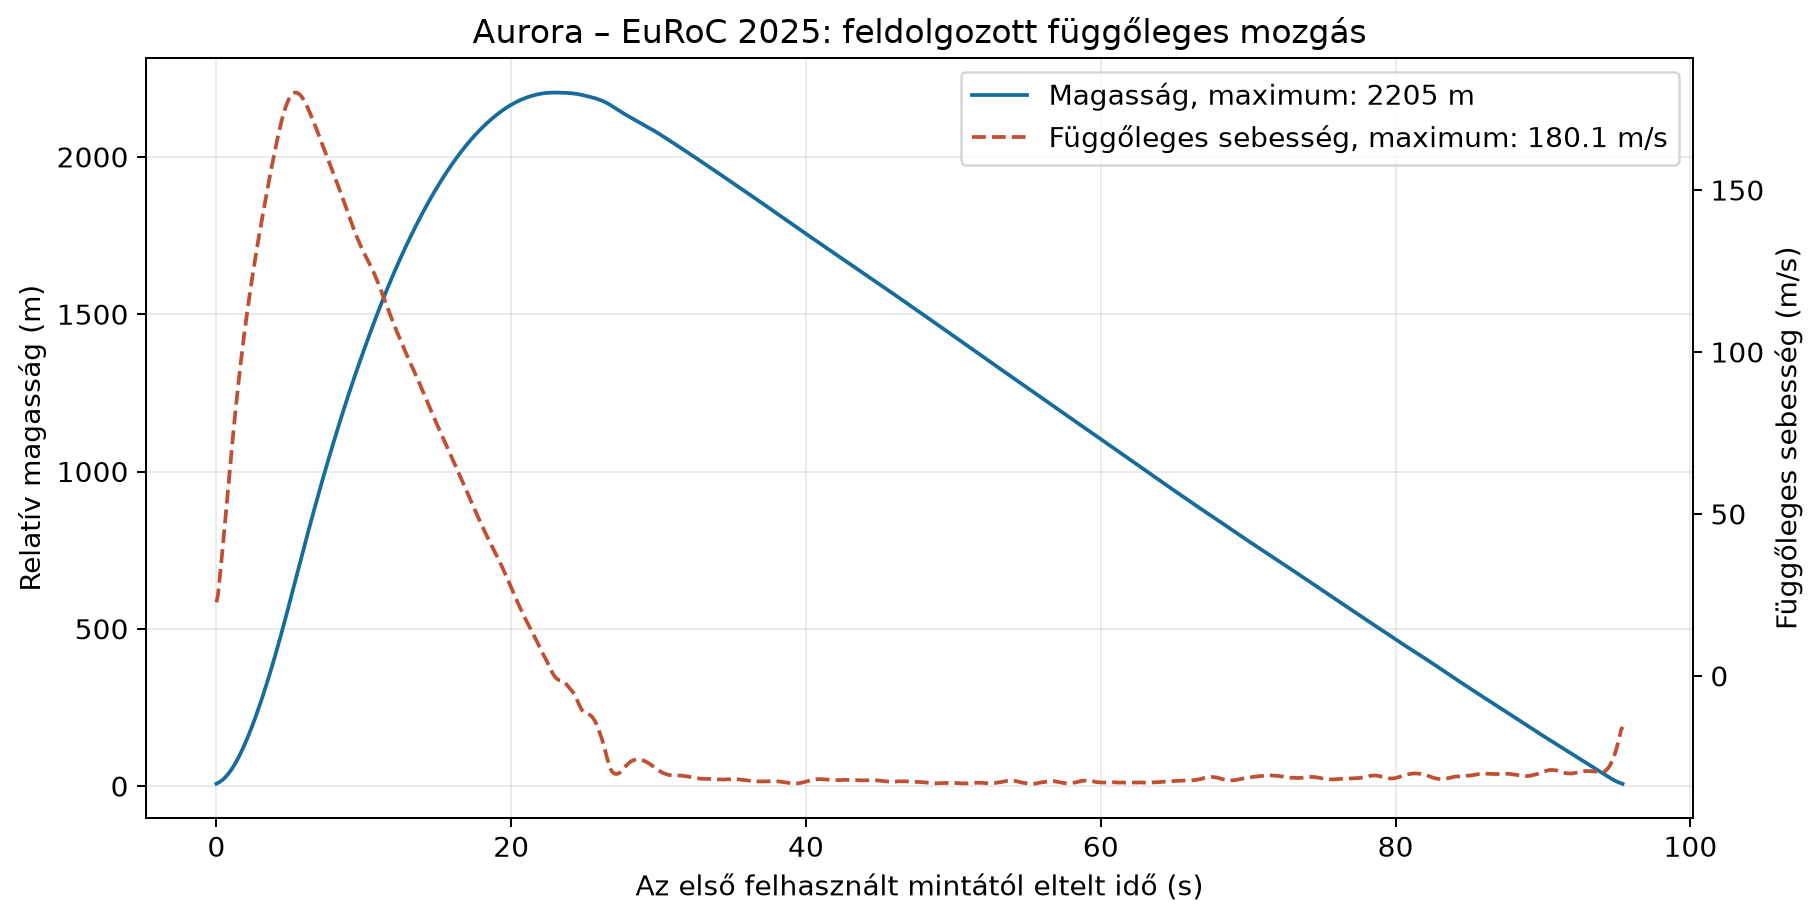
\includegraphics[width=\textwidth]{figures/Requirements/aurora_euroc_cats_flight_profile.png}
    \caption{Az Aurora rakéta függőleges repülési profilja a 2025-ös EuRoC során}
    \label{fig:aurora-euroc-flight-profile}
\end{figure}

A vízszintes elmozdulásokat a földrajzi koodrinátákból helyi,
kelet és északi irányú koordinátarendszerbe lettek transzformálva.
Az alábbbi közelítés lett alkalmazva a vizsgált távolságokon:
\cite{equirectangular-projection}:
\begin{align}
    E(t) &= R_{\mathrm{F}}\cos\varphi_0
    \bigl(\lambda(t)-\lambda_0\bigr) \\
    N(t) &= R_{\mathrm{F}}
    \bigl(\varphi(t)-\varphi_0\bigr)
\end{align}
ahol $\lambda$ a földrajzi hosszúság, $\varphi$ a földrajzi szélesség,
$\lambda_0$ és $\varphi_0$ az első felhasznált pozíció koordinátái,
$R_{\mathrm{F}}=6\,378\,137~\mathrm{m}$  pedig az alkalmazott
földsugár.
Az $E$ koordináta keleti, az $N$ koordináta északi irányú
elmozdulást jelöl. 

Azonban a GPS adatsorban több ismétlödő adat és hirtelen koordinátaugrások
is előfordultak. Ezek numerikus deriválással irreális eredményeket adtak.
Ezért a kezdeti referenciahely és az első felhasználható
GPS-pozíció közötti hiányzó pályaszakaszt harmadfokú
polinommal lett közelítve, a két végpontban nulla vízszintes sebességet feltételezve. 
Emellett az utolsó felhasznlt GPS pozicíó  után a motgást a megelöző GPS
szakaszból becsült állandó sebességgel lett közelítve.

Így a rekonstoktuált pályabecslés a következő árbráról \ref{fig:aurora-euroc-horizontal-drift} leolvasható:
\begin{figure}[H]
    \centering
    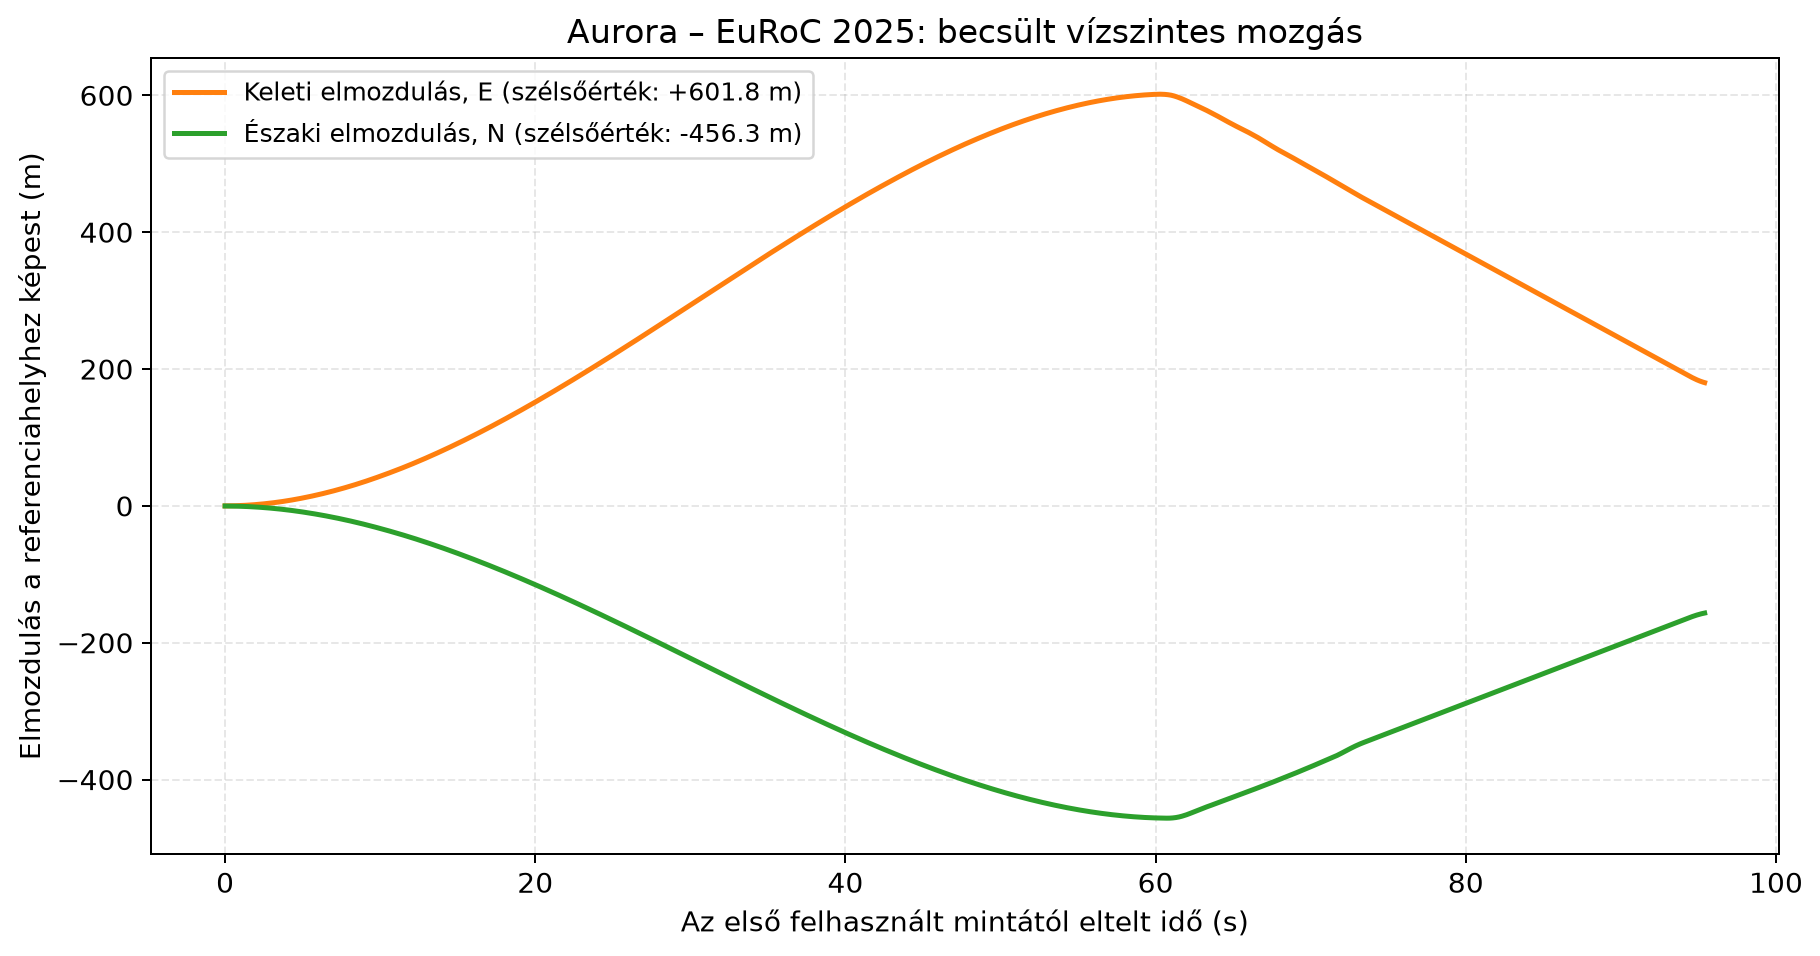
\includegraphics[width=\textwidth]{figures/Requirements/aurora_euroc_cats_horizontal_drift.png}
    \caption{Az Aurora rakéta vízszintes elmozdulása és sodródása a 2025-ös EuRoC során}
    \label{fig:aurora-euroc-horizontal-drift}
\end{figure}


Az Eclipse integrált repülési tesztjének pályabevcslését az CATs által rögzített
magasság és sebességadatokból, illetve IMU adatokból lett meghatározva. \\

Az Eclipse függőleges mozgásprofilja a CATS által exportált
magasság- és függőlegessebesség-adatokon alapul.
A mozgásprofilt a \ref{fig:eclipse-ift-flight-profile}.~ábra mutatja be:
\begin{figure}[H]
    \centering
    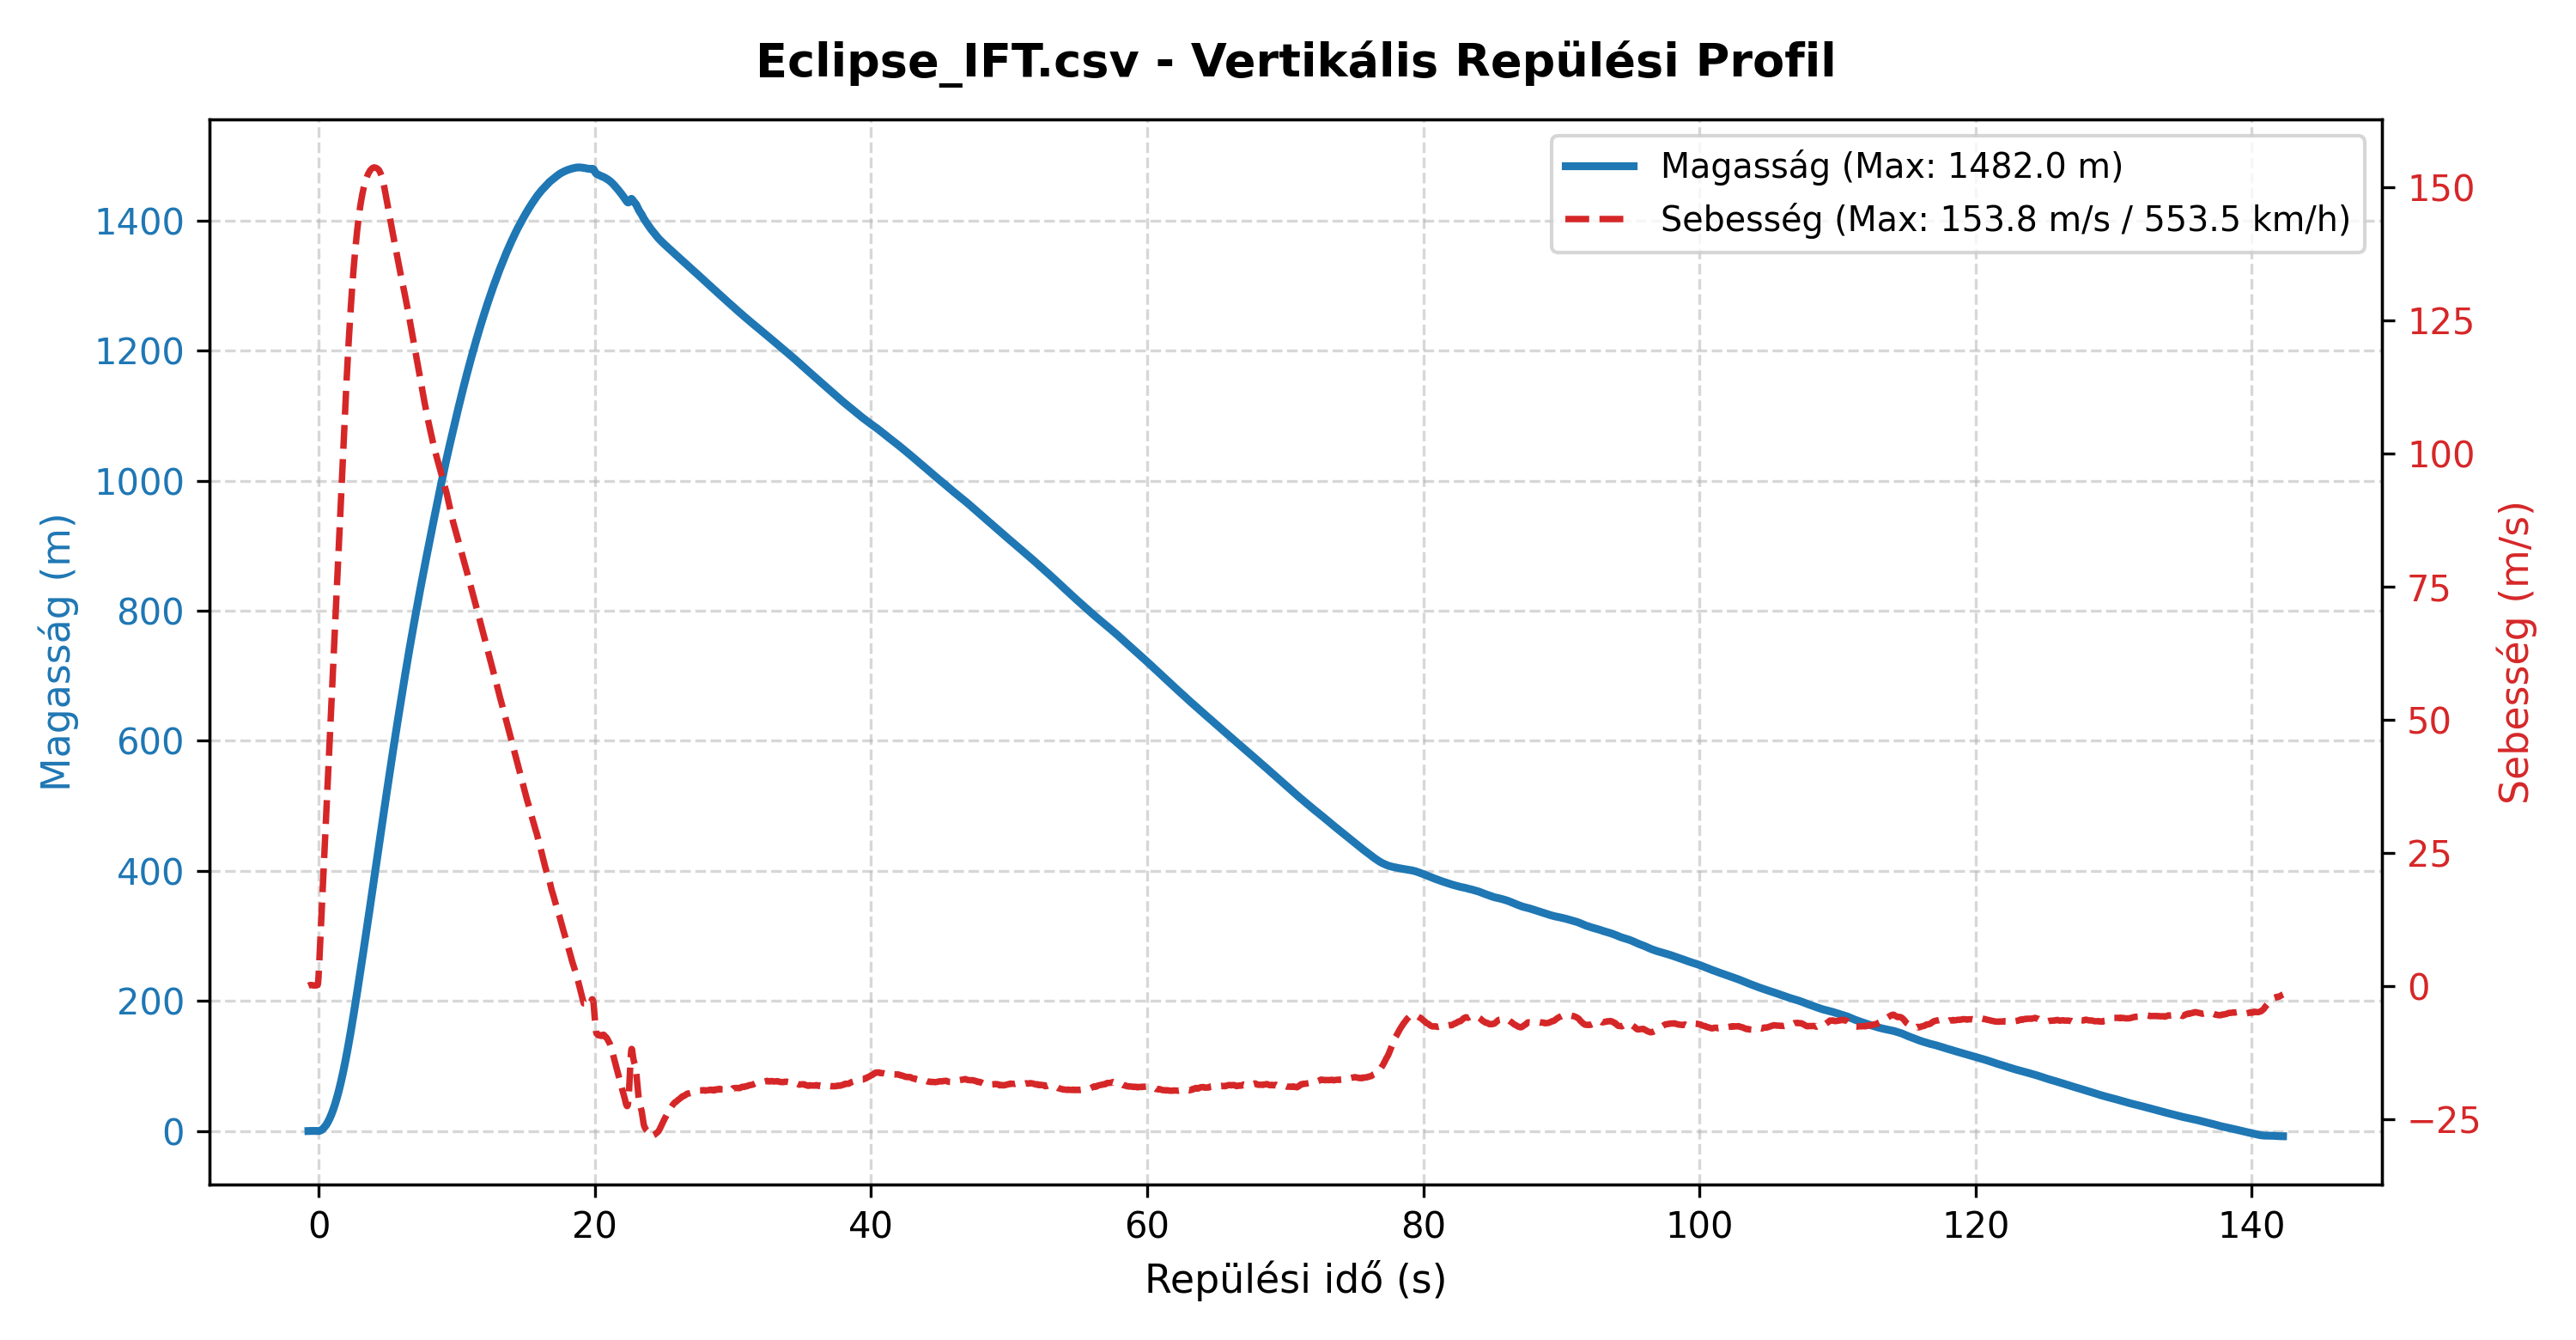
\includegraphics[width=\textwidth]{figures/Requirements/eclipse_ift_flight_profile.png}
    \caption{Az Eclipse rakéta függőleges repülési profilja az IFT során}
    \label{fig:eclipse-ift-flight-profile}
\end{figure}

A vízszintes elmozdulását az IMU adatok feldolgozásával lett megbecsülve.
A számítás során a giroszkóp nullponti eltolódást az indítós előtt mért adatok
alapján lett korrigálva, melyet a repülési adatokból levonásra kerültek. 
A korrigált szögsebességekből a rakéta oriontációja mintánként frissttve.
A helyi koordinátarendszerve forgatott és gravitécióval kompenzált 
gyorsulás integrálásából adoódik a vizszintes sebességek, illetve
azok integrálásából a vízszintes elmozdulások.
A becsült vízszintes elmozdulásokat
a \ref{fig:eclipse-ift-horizontal-drift}.~ábra mutatja:
\begin{figure}[H]
    \centering
    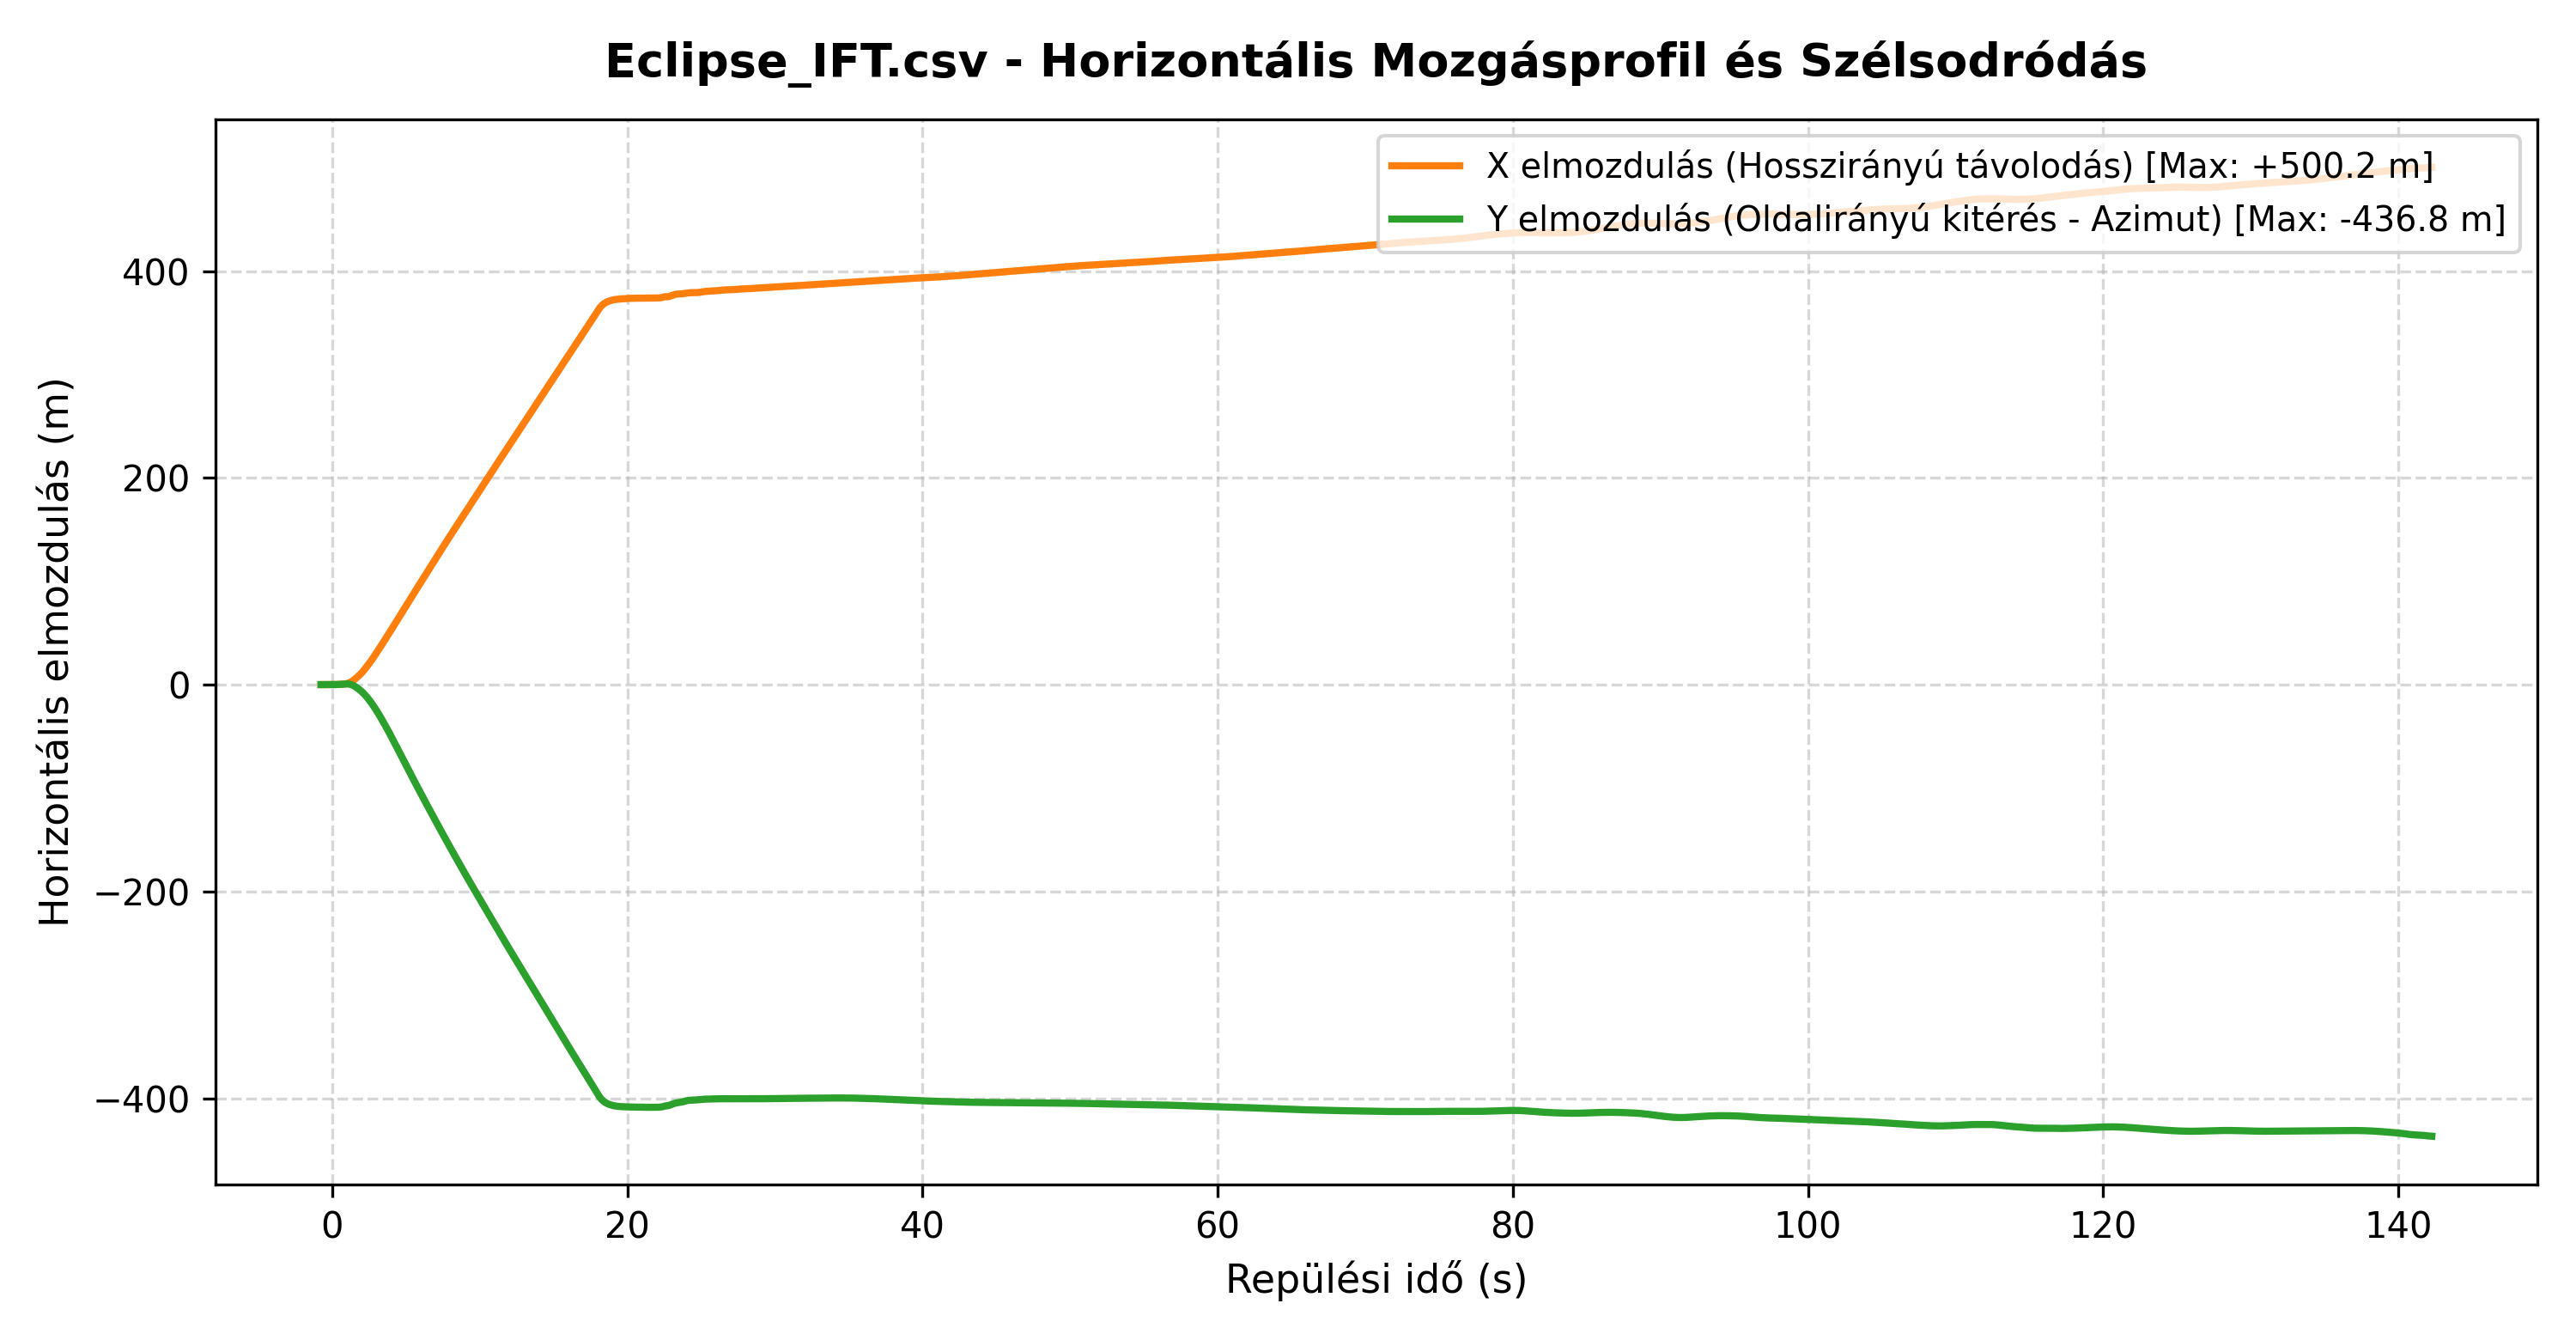
\includegraphics[width=\textwidth]{figures/Requirements/eclipse_ift_horizontal_drift.png}
    \caption{Az Eclipse rakéta vízszintes elmozdulása és sodródása az IFT során}
    \label{fig:eclipse-ift-horizontal-drift}
\end{figure}


\subsubsection{Szükséges szögelfordulások, szögsebességek és szöggyorsulások meghatározása}
\label{subsubsec:antenna-seb}

Az elöző alfejezetben \ref{subsubsec:szogsebesseg-szoggyorsulas} meghatározott
repülési adatokból meghatározható, hogy a rakéta követéséhez a földi követőállomásnak antennjának
adott távolságokban, milyen vízszintes és függőleges szögelfordulásara, szögsebességere és szöggyorsulásra van szüksége.
A vizsgált földiállomás-távolságok 500~m és 1500~m között,
250~m-es lépésekben kerültek meghatározásra.

A helyi koordinátarendszer origója a rakéta indítási helye, a $z$ tengely
függőlegesen felfelé mutat,  míg a pozitív $x$ tengely a kijelölt biztonsági lőirány. 
A biztonsági előírásoknak megfelelően a földi
állomást és az irányító személyzetet a lőiránnyal elentétesen, azaz $x$ tengely negatív
irányában, $D$ biztonsági távolságra kell elhelyezni, garantálva, hogy a rakéta a fellövés
pillanatától kezdve mindig távolodjon az állomástól a fellövés során. Így az állomás 
helyvektora a következő:
\begin{equation}
    \boldsymbol{r}_{\mathrm{f}}
    = \begin{bmatrix} -D \\ 0 \\ 0 \end{bmatrix}
    \label{eq:kovetes-foldi-pozicio}
\end{equation}

A raakéta és a földi állomás közötti vízszintes távolság:
\begin{equation}
    \boldsymbol{r}_{\mathrm{rel}}(t)
    = \boldsymbol{r}_{\mathrm{r}}(t)-\boldsymbol{r}_{\mathrm{f}}
    = \begin{bmatrix}
        X_{\mathrm{r}}(t)-(-D) \\
        Y_{\mathrm{r}}(t) \\
        Z_{\mathrm{r}}(t)
      \end{bmatrix}
    = \begin{bmatrix}
        X_{\mathrm{r}}(t)+D \\
        Y_{\mathrm{r}}(t) \\
        Z_{\mathrm{r}}(t)
      \end{bmatrix}
    = \begin{bmatrix}
        x_{\mathrm{rel}}(t) \\
        y_{\mathrm{rel}}(t) \\
        z_{\mathrm{rel}}(t)
      \end{bmatrix}
    \label{eq:kovetes-relativ-pozicio}
\end{equation}


Mivel a földi állomás helyzete állandó, a relatív helyvektor idő szerinti
deriváltja megegyezik a rakéta sebességvektorvél:
\begin{equation}
    \boldsymbol{v}_{\mathrm{rel}}
    = \dot{\boldsymbol{r}}_{\mathrm{rel}}
    = \boldsymbol{v}_{\mathrm{r}}
    = \begin{bmatrix} v_x \\ v_y \\ v_z \end{bmatrix}
    \label{eq:kovetes-relativ-sebesseg}
\end{equation}

A rakéta és a földi állomás közötti vízszintes távolság
a relatív helyvektor vízszintes vetületének hossza:
\begin{equation}
    d_{\mathrm{rel}}
    = \sqrt{x_{\mathrm{rel}}^2+y_{\mathrm{rel}}^2}
    \label{eq:kovetes-vizszintes-tavolsag}
\end{equation}


Az antenna elevációs szöge a rakéta felé mutató irány
vízszintes síkhoz képest mért szöge. Ha $d_{\mathrm{rel}}>0$,
akkor
\begin{equation}
    \theta = \arctan\!\left(\frac{z_{\mathrm{rel}}}{d_{\mathrm{rel}}}\right)
    \label{eq:kovetes-elevacio}
\end{equation}

Az elevációs szögsebesség meghatározásához szükséges a vízszintes
távolság idő szerinti deriváltja:
\begin{align}
    \dot{d}_{\mathrm{rel}}
    &= \dfrac{\partial d_{rel}}{\partial x_{rel}}\cdot \dfrac{d x_{rel}}{d t}
       + \dfrac{\partial d_{rel}}{\partial y_{rel}} \cdot \dfrac{d y_{rel}}{d t} \\
    & = \dfrac{2x_\mathrm{rel}}{2\sqrt{x_{\mathrm{rel}}^2+y_{\mathrm{rel}}^2}}
       \cdot v_x+ + \dfrac{2y_\mathrm{rel}}{2\sqrt{x_{\mathrm{rel}}^2+y_{\mathrm{rel}}^2}}
       \cdot v_y \\
    &= \frac{x_{\mathrm{rel}}v_x+y_{\mathrm{rel}}v_y}{d_{\mathrm{rel}}}
    \label{eq:kovetes-vizszintes-sebesseg}
\end{align}


Az \eqref{eq:kovetes-elevacio} egyenlet idő szerinti
deriválásából, a láncszabály és a hányados deriválási
szabályának alkalmazásával adódik az elevációs szögsebesség:
\begin{equation}
    \begin{aligned}
        \dot{\theta}
        &= \frac{1}{1+\left(z_{\mathrm{rel}}/d_{\mathrm{rel}}\right)^2}
           \frac{\mathrm{d}}{\mathrm{d}t}
           \left(\frac{z_{\mathrm{rel}}}{d_{\mathrm{rel}}}\right) \\
        &= \frac{d_{\mathrm{rel}}^2}
                {d_{\mathrm{rel}}^2+z_{\mathrm{rel}}^2}
           \frac{d_{\mathrm{rel}}v_z-z_{\mathrm{rel}}\dot{d}_{\mathrm{rel}}}
                {d_{\mathrm{rel}}^2} \\
        &= \frac{d_{\mathrm{rel}}v_z-z_{\mathrm{rel}}\dot{d}_{\mathrm{rel}}}
                {d_{\mathrm{rel}}^2+z_{\mathrm{rel}}^2}
    \end{aligned}
    \label{eq:kovetes-elevacios-szogsebesseg}
\end{equation}

Az elevációs szöggyorsulás a szögsebesség numerikus deriválásával adódik. 
Egyenletes mintavétel esetén másodrendű centrális differenciával közelíthető:
\begin{align}
    \ddot{\theta} = \dfrac{d \dot{\theta}}{dt} \approx \dfrac{\dot{theta}(t+\Delta t)-\dot{\theta}(t-\Delta t)}{\Delta t}
\label{eq:kovetes-elevacios-szoggyorsulas}
\end{align}

Az azimutszög a rakéta felé mutató relatív helyvektor vízszintes vetületének irányszöge,
$x$ tengely pozitív irányától az $y$ tengely pozitív
iránya felé mérve.  A megfelelő síknegyed figyelembevételéhez
az atan2 függvény alkalmazható:
\begin{equation}
    \psi = \operatorname{atan2}(y_{\mathrm{rel}},x_{\mathrm{rel}})
    \label{eq:kovetes-azimut}
\end{equation}

Az azimutszög idő szerinti deriváltja:
\begin{equation}
    \dot{\psi}
    = \frac{x_{\mathrm{rel}}v_y-y_{\mathrm{rel}}v_x}
           {x_{\mathrm{rel}}^2+y_{\mathrm{rel}}^2}
    \label{eq:kovetes-azimut-szogsebesseg}
\end{equation}


A szögsebességek ezekből az összefüggésekből radián/másodperc
mértékegységben adódnak. 
Ebből a szögsebességből a szöggyorsulás meghatározható, amelyet hasonlóan a 
\ref{eq:kovetes-elevacios-szoggyorsulas} egyenlethez, numerikus deriválással és
másodrendú centrális differenciálhányados közelítéssel kapjuk meg:
\begin{align}
    \ddot{\psi} = \dfrac{d \dot{\psi}}{dt} \approx \dfrac{\dot{\psi}(t+\Delta t)-\dot{\psi}(t-\Delta t)}{\Delta t}
\label{eq:kovetes-azimut-szoggyorsulas}
\end{align}

A \ref{fig:eclipse-ift-elev-tracking}. és a
\ref{fig:aurora-euroc-cats-elev-tracking}.~ábra az Eclipse és
az Aurora követéséhez szükséges elevációs szöget,
szögsebességet és szöggyorsulást mutatja a különböző
állomástávolságokra:

\begin{figure}[H]
    \centering
    \begin{minipage}[t]{0.48\textwidth}
        \centering
        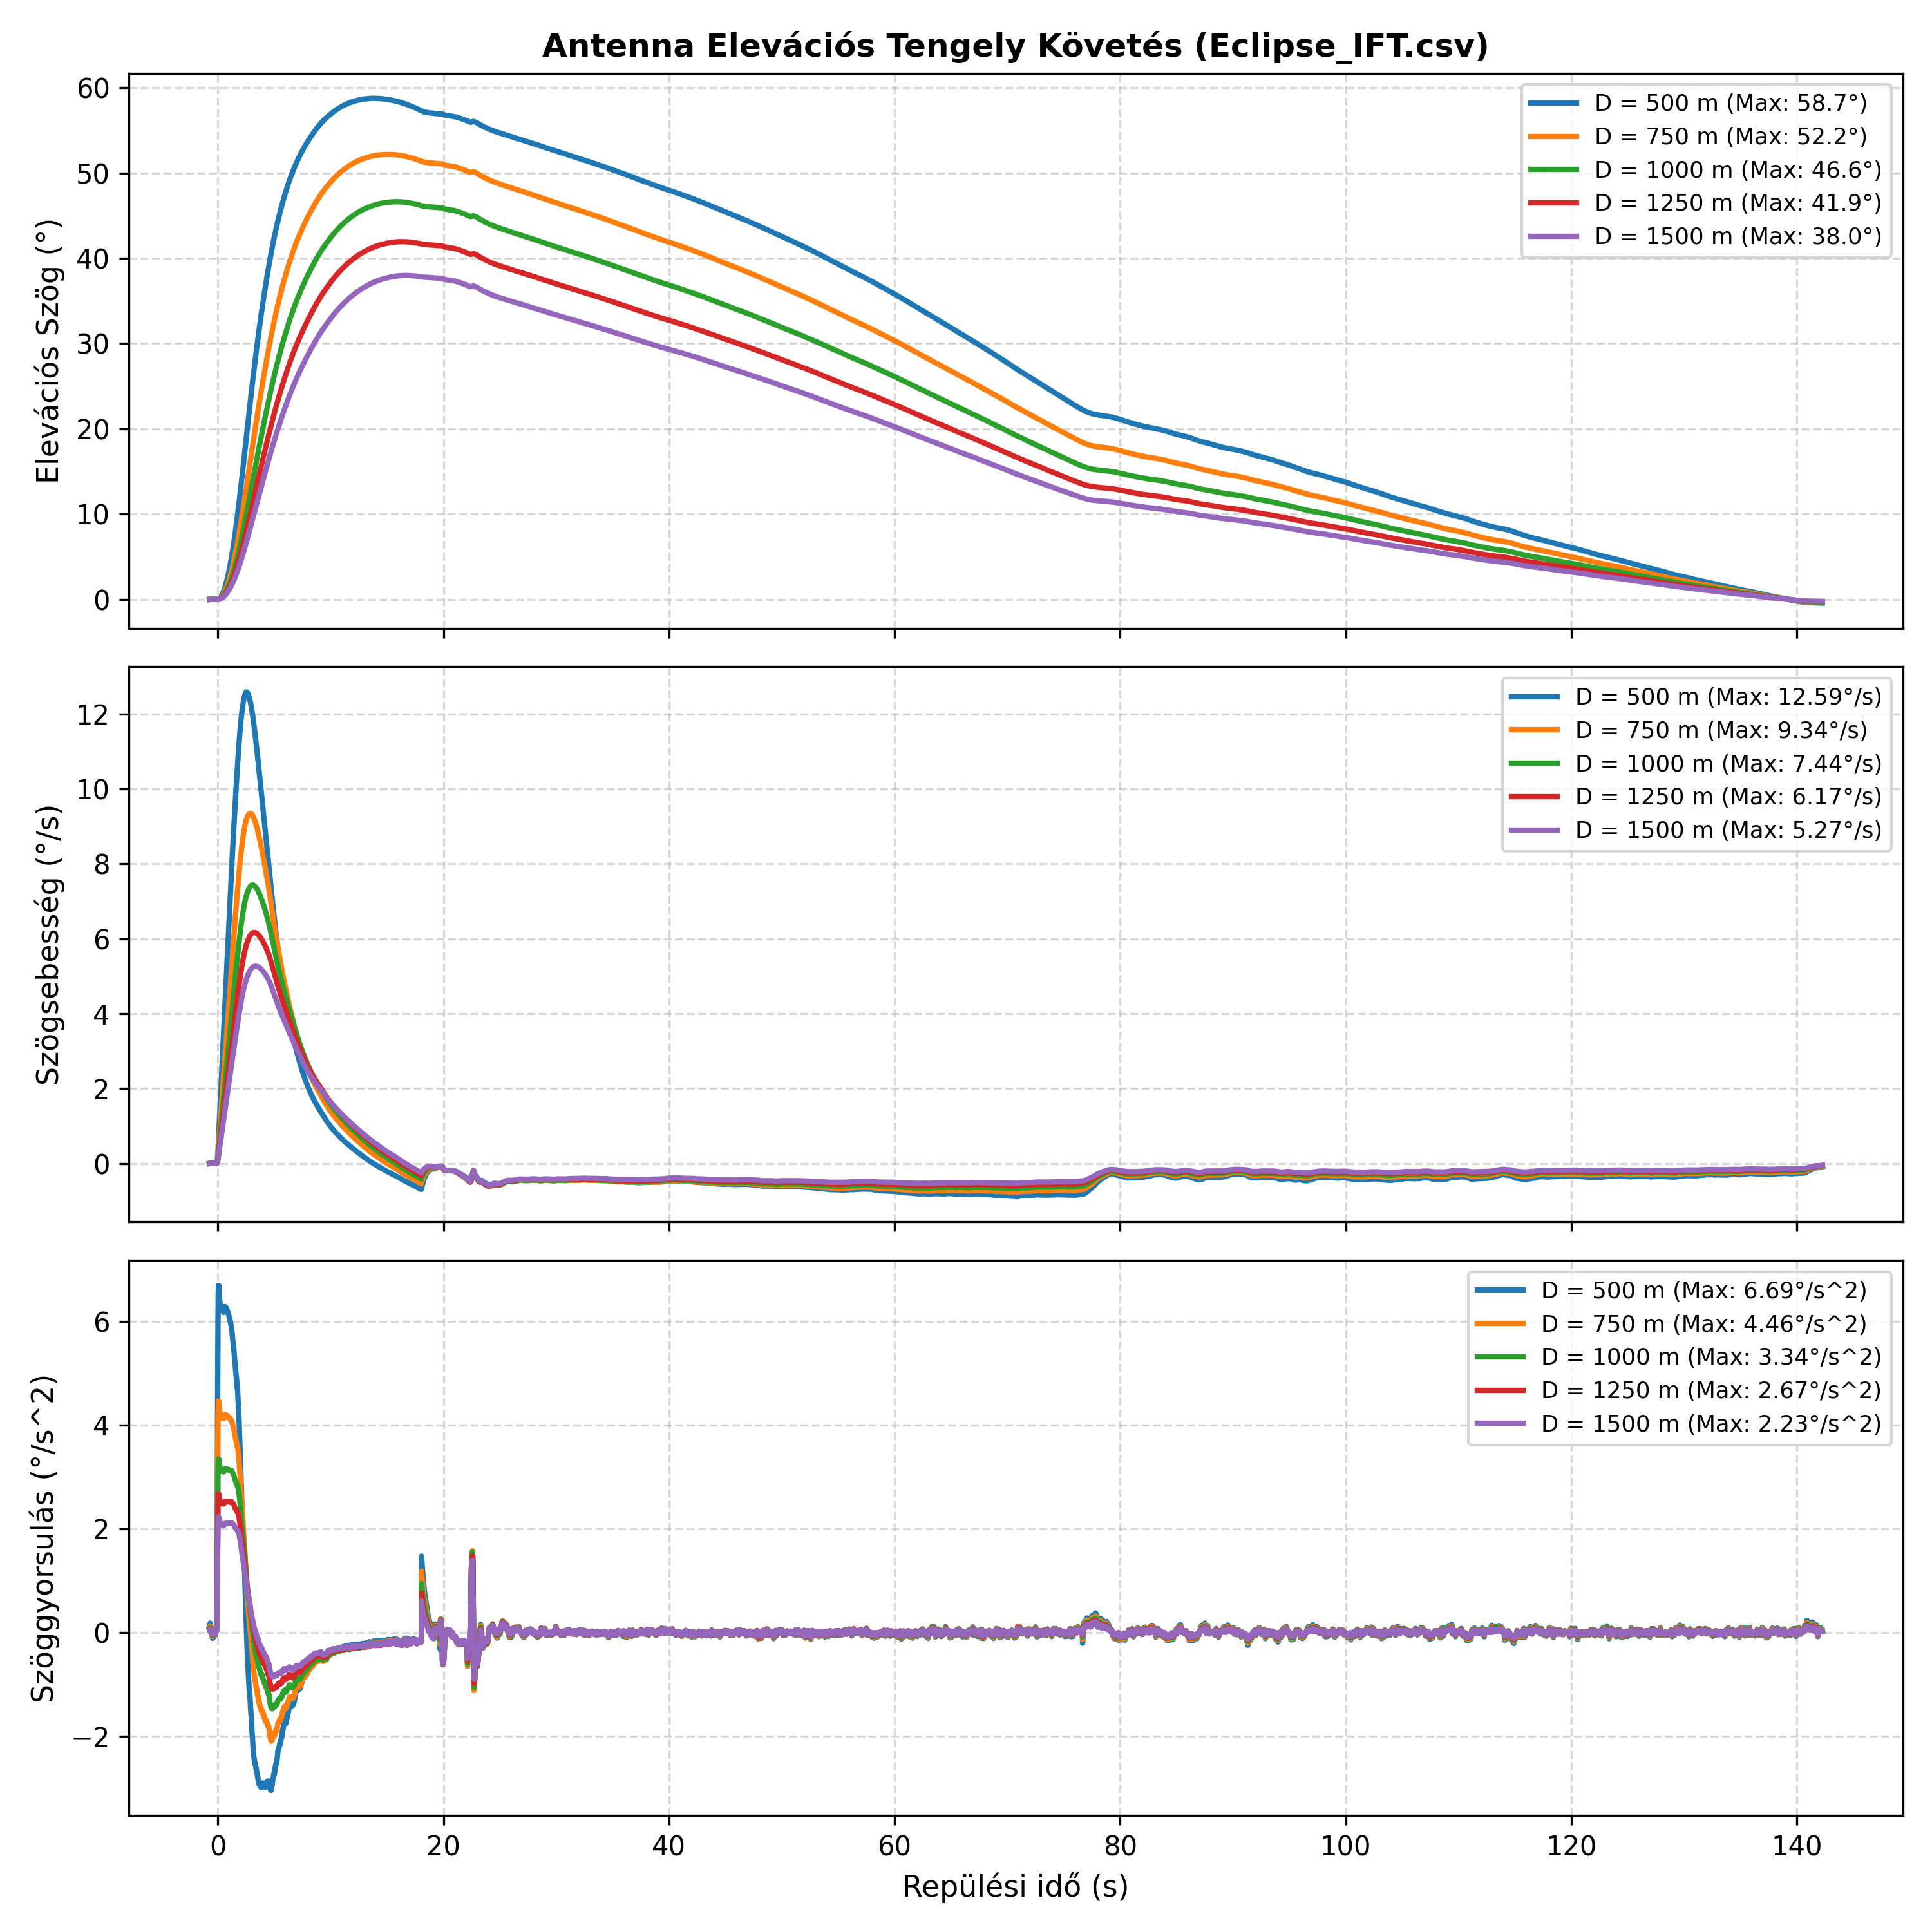
\includegraphics[width=\linewidth]{figures/Requirements/eclipse_ift_elev_tracking.png}
        \captionsetup{width=\linewidth,format=plain,justification=centering}
        \caption{Az Eclipse elevációkövetése az IFT során}
        \label{fig:eclipse-ift-elev-tracking}
    \end{minipage}\hfill
    \begin{minipage}[t]{0.48\textwidth}
        \centering
        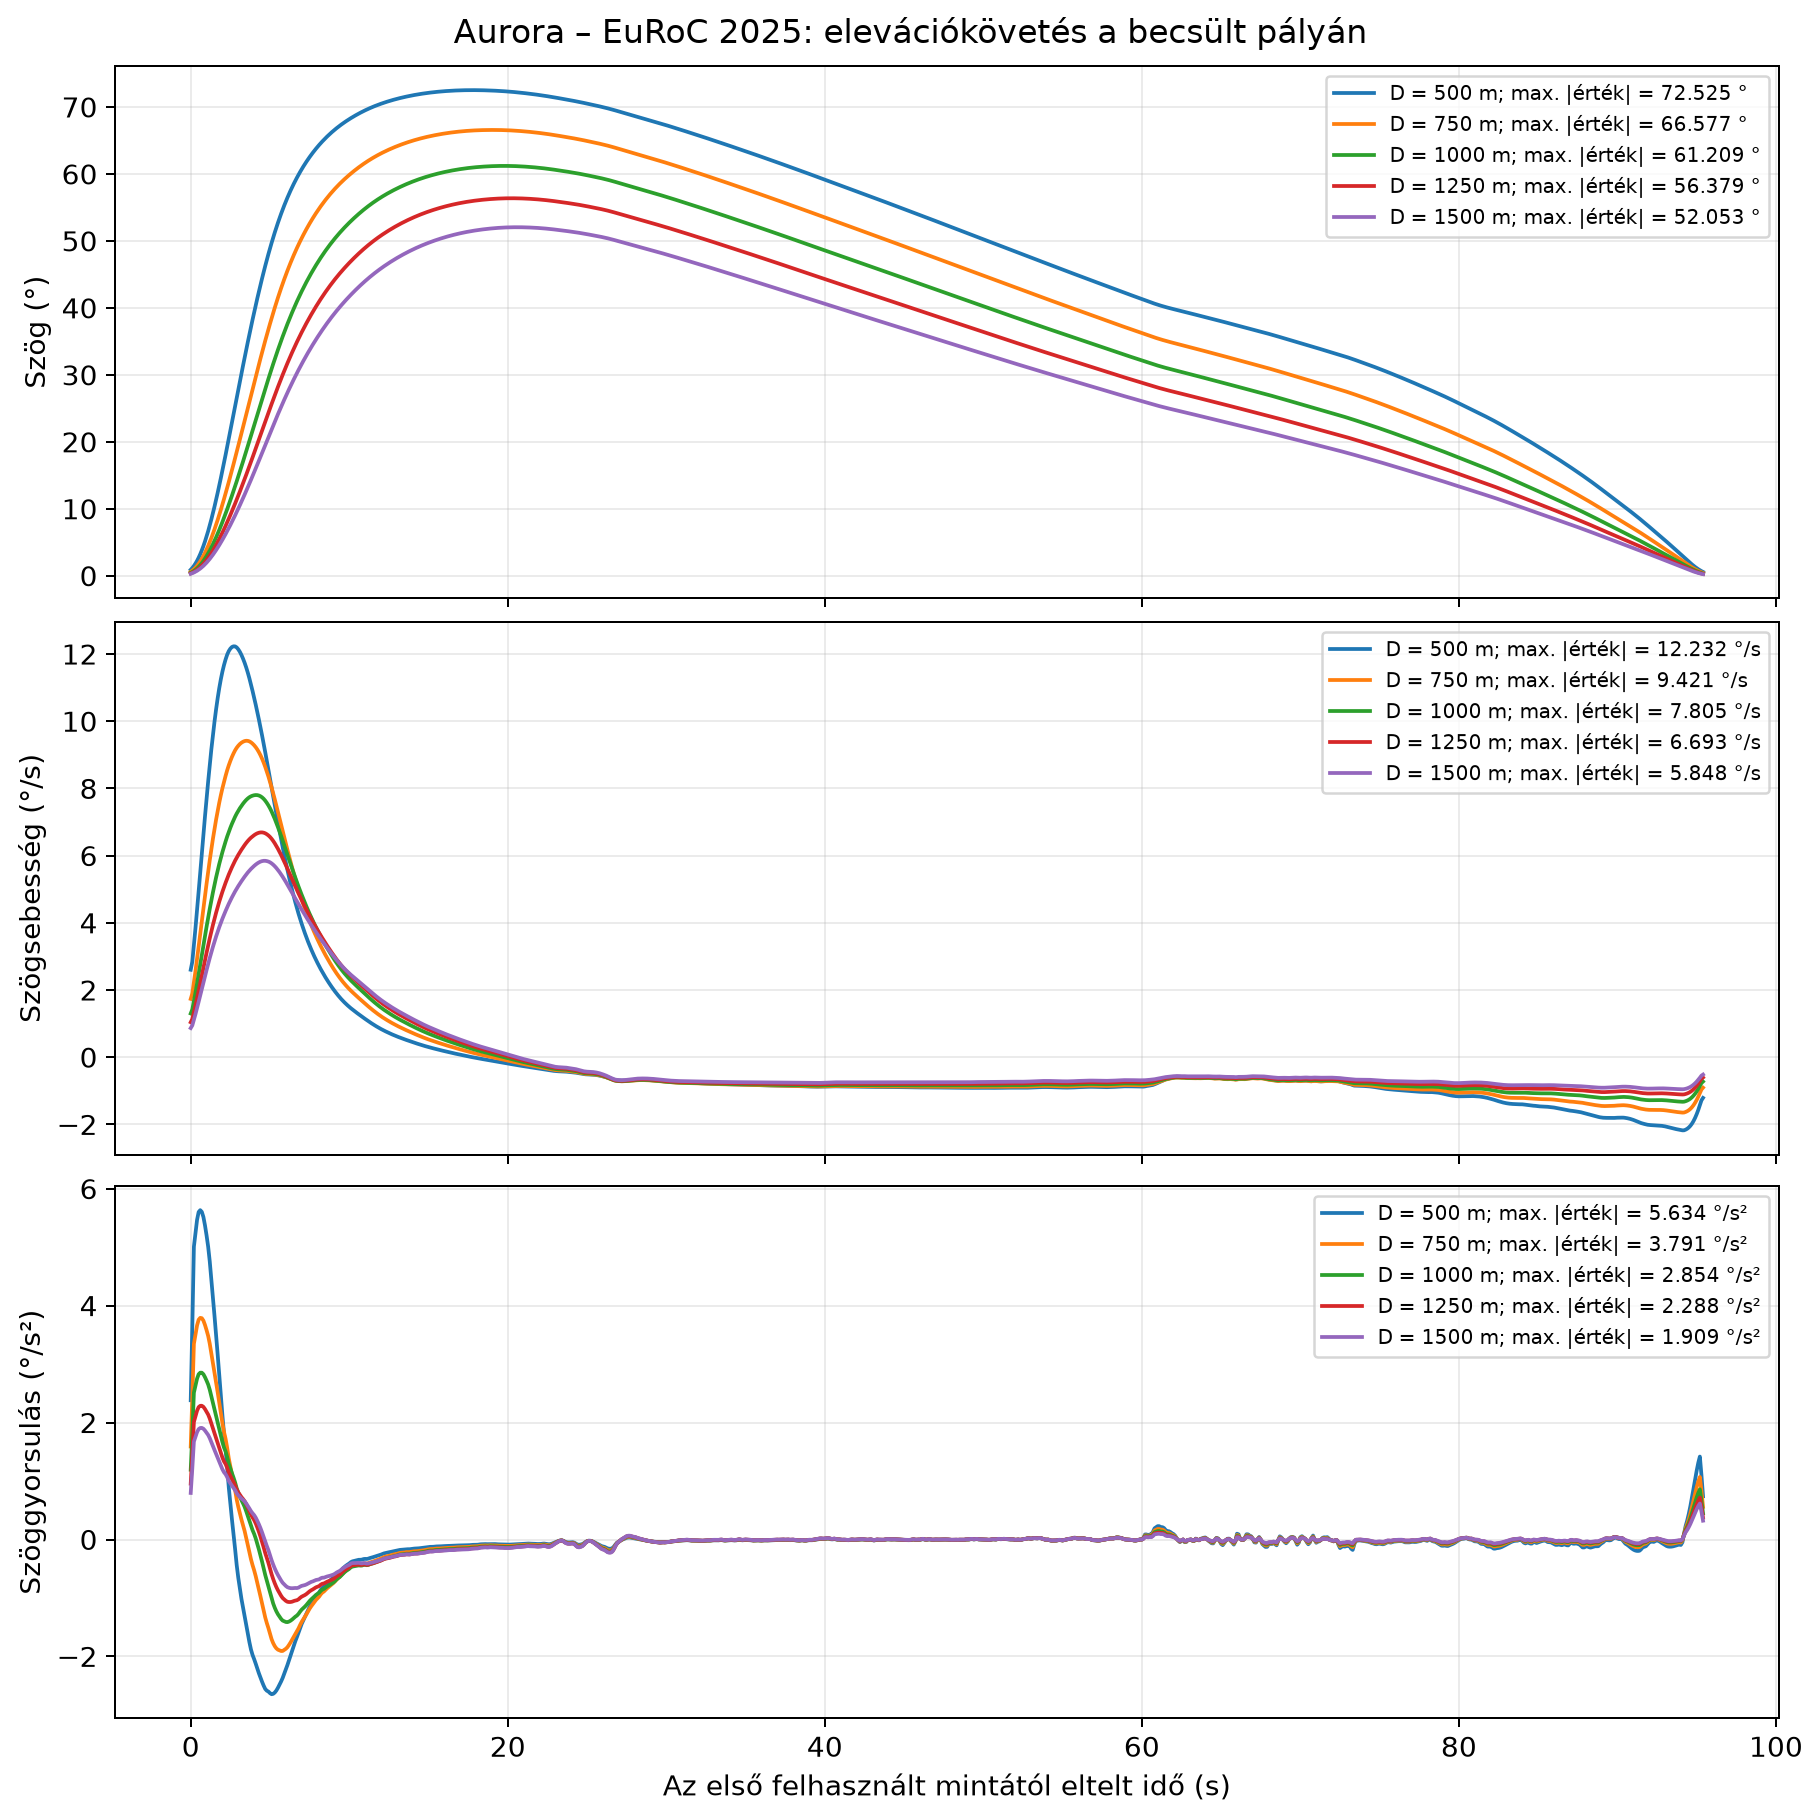
\includegraphics[width=\linewidth]{figures/Requirements/aurora_euroc_cats_elev_tracking.png}
        \captionsetup{width=\linewidth,format=plain,justification=centering}
        \caption{Az Aurora elevációkövetése a 2025-ös EuRoC során}
        \label{fig:aurora-euroc-cats-elev-tracking}
    \end{minipage}
\end{figure}

Az azimutszög, az azimut-szögsebesség és az
azimut-szöggyorsulás időbeli alakulását a
\ref{fig:eclipse-ift-azim-tracking}. és a
\ref{fig:aurora-euroc-cats-azim-tracking}.~ábra mutatja:

\begin{figure}[H]
    \centering
    \begin{minipage}[t]{0.48\textwidth}
        \centering
        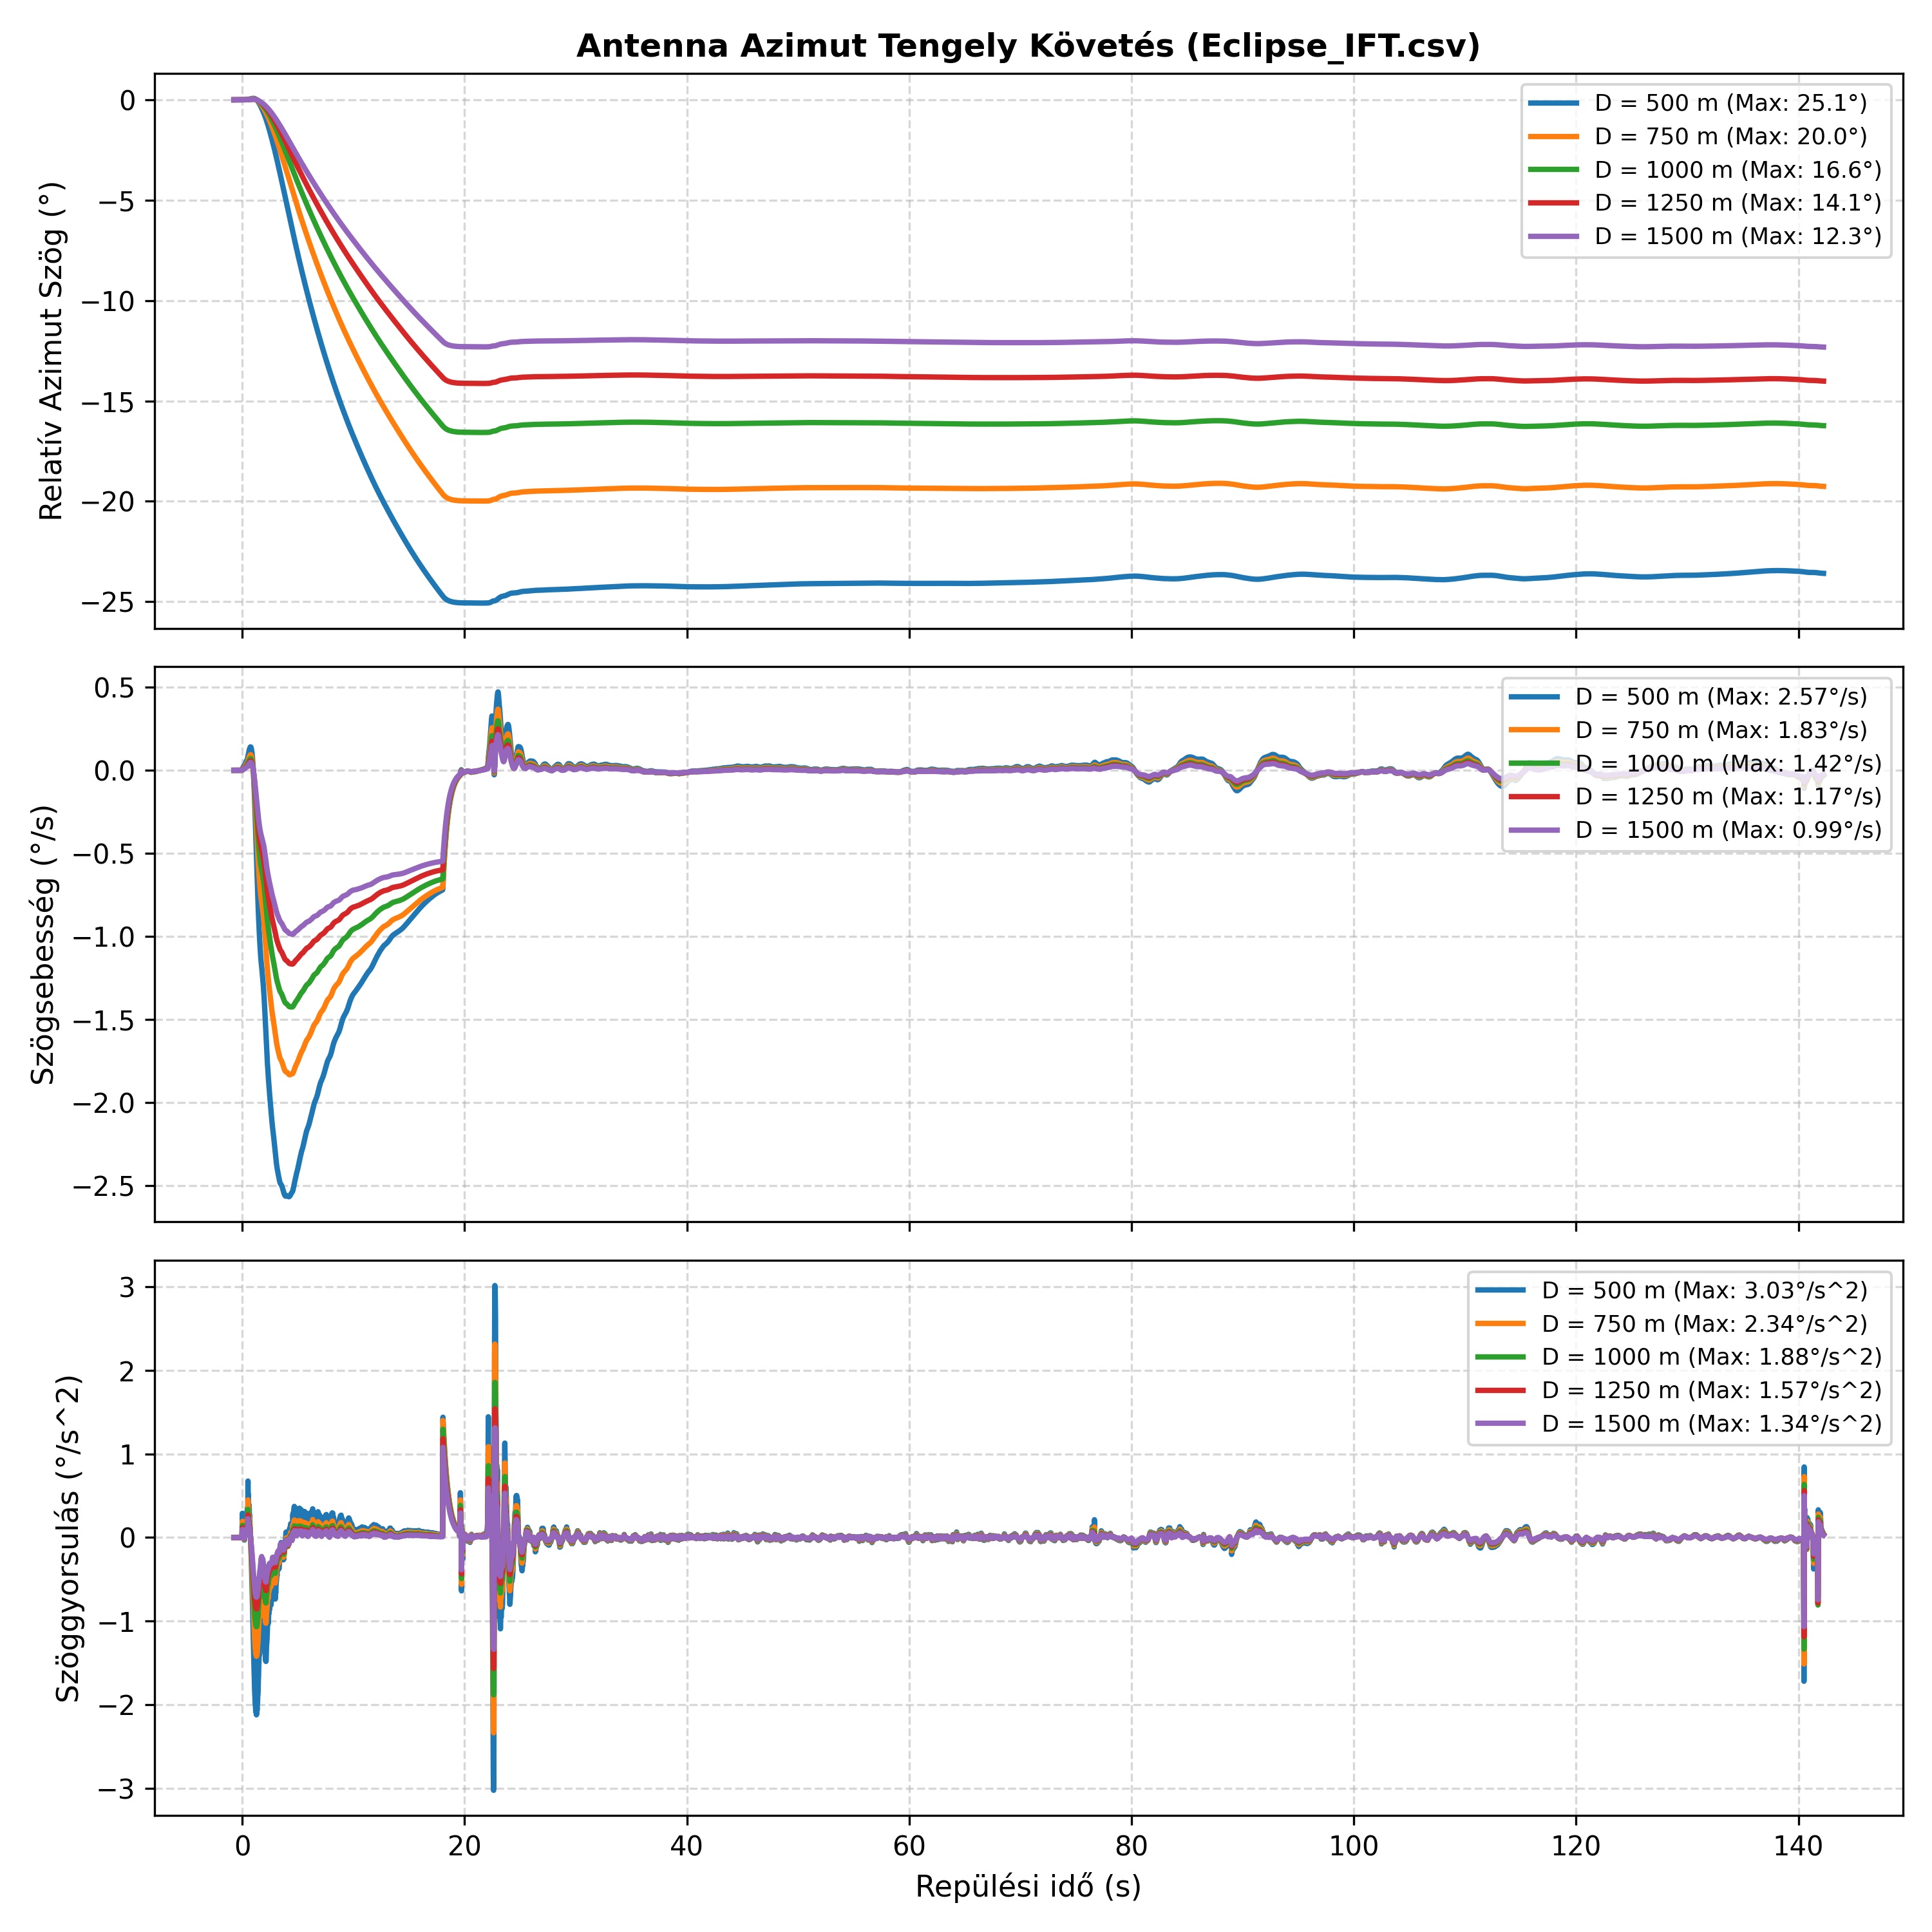
\includegraphics[width=\linewidth]{figures/Requirements/eclipse_ift_azimuth_tracking.png}
        \captionsetup{width=\linewidth,format=plain,justification=centering}
        \caption{Az Eclipse azimutkövetése az IFT során}
        \label{fig:eclipse-ift-azim-tracking}
    \end{minipage}\hfill
    \begin{minipage}[t]{0.48\textwidth}
        \centering
        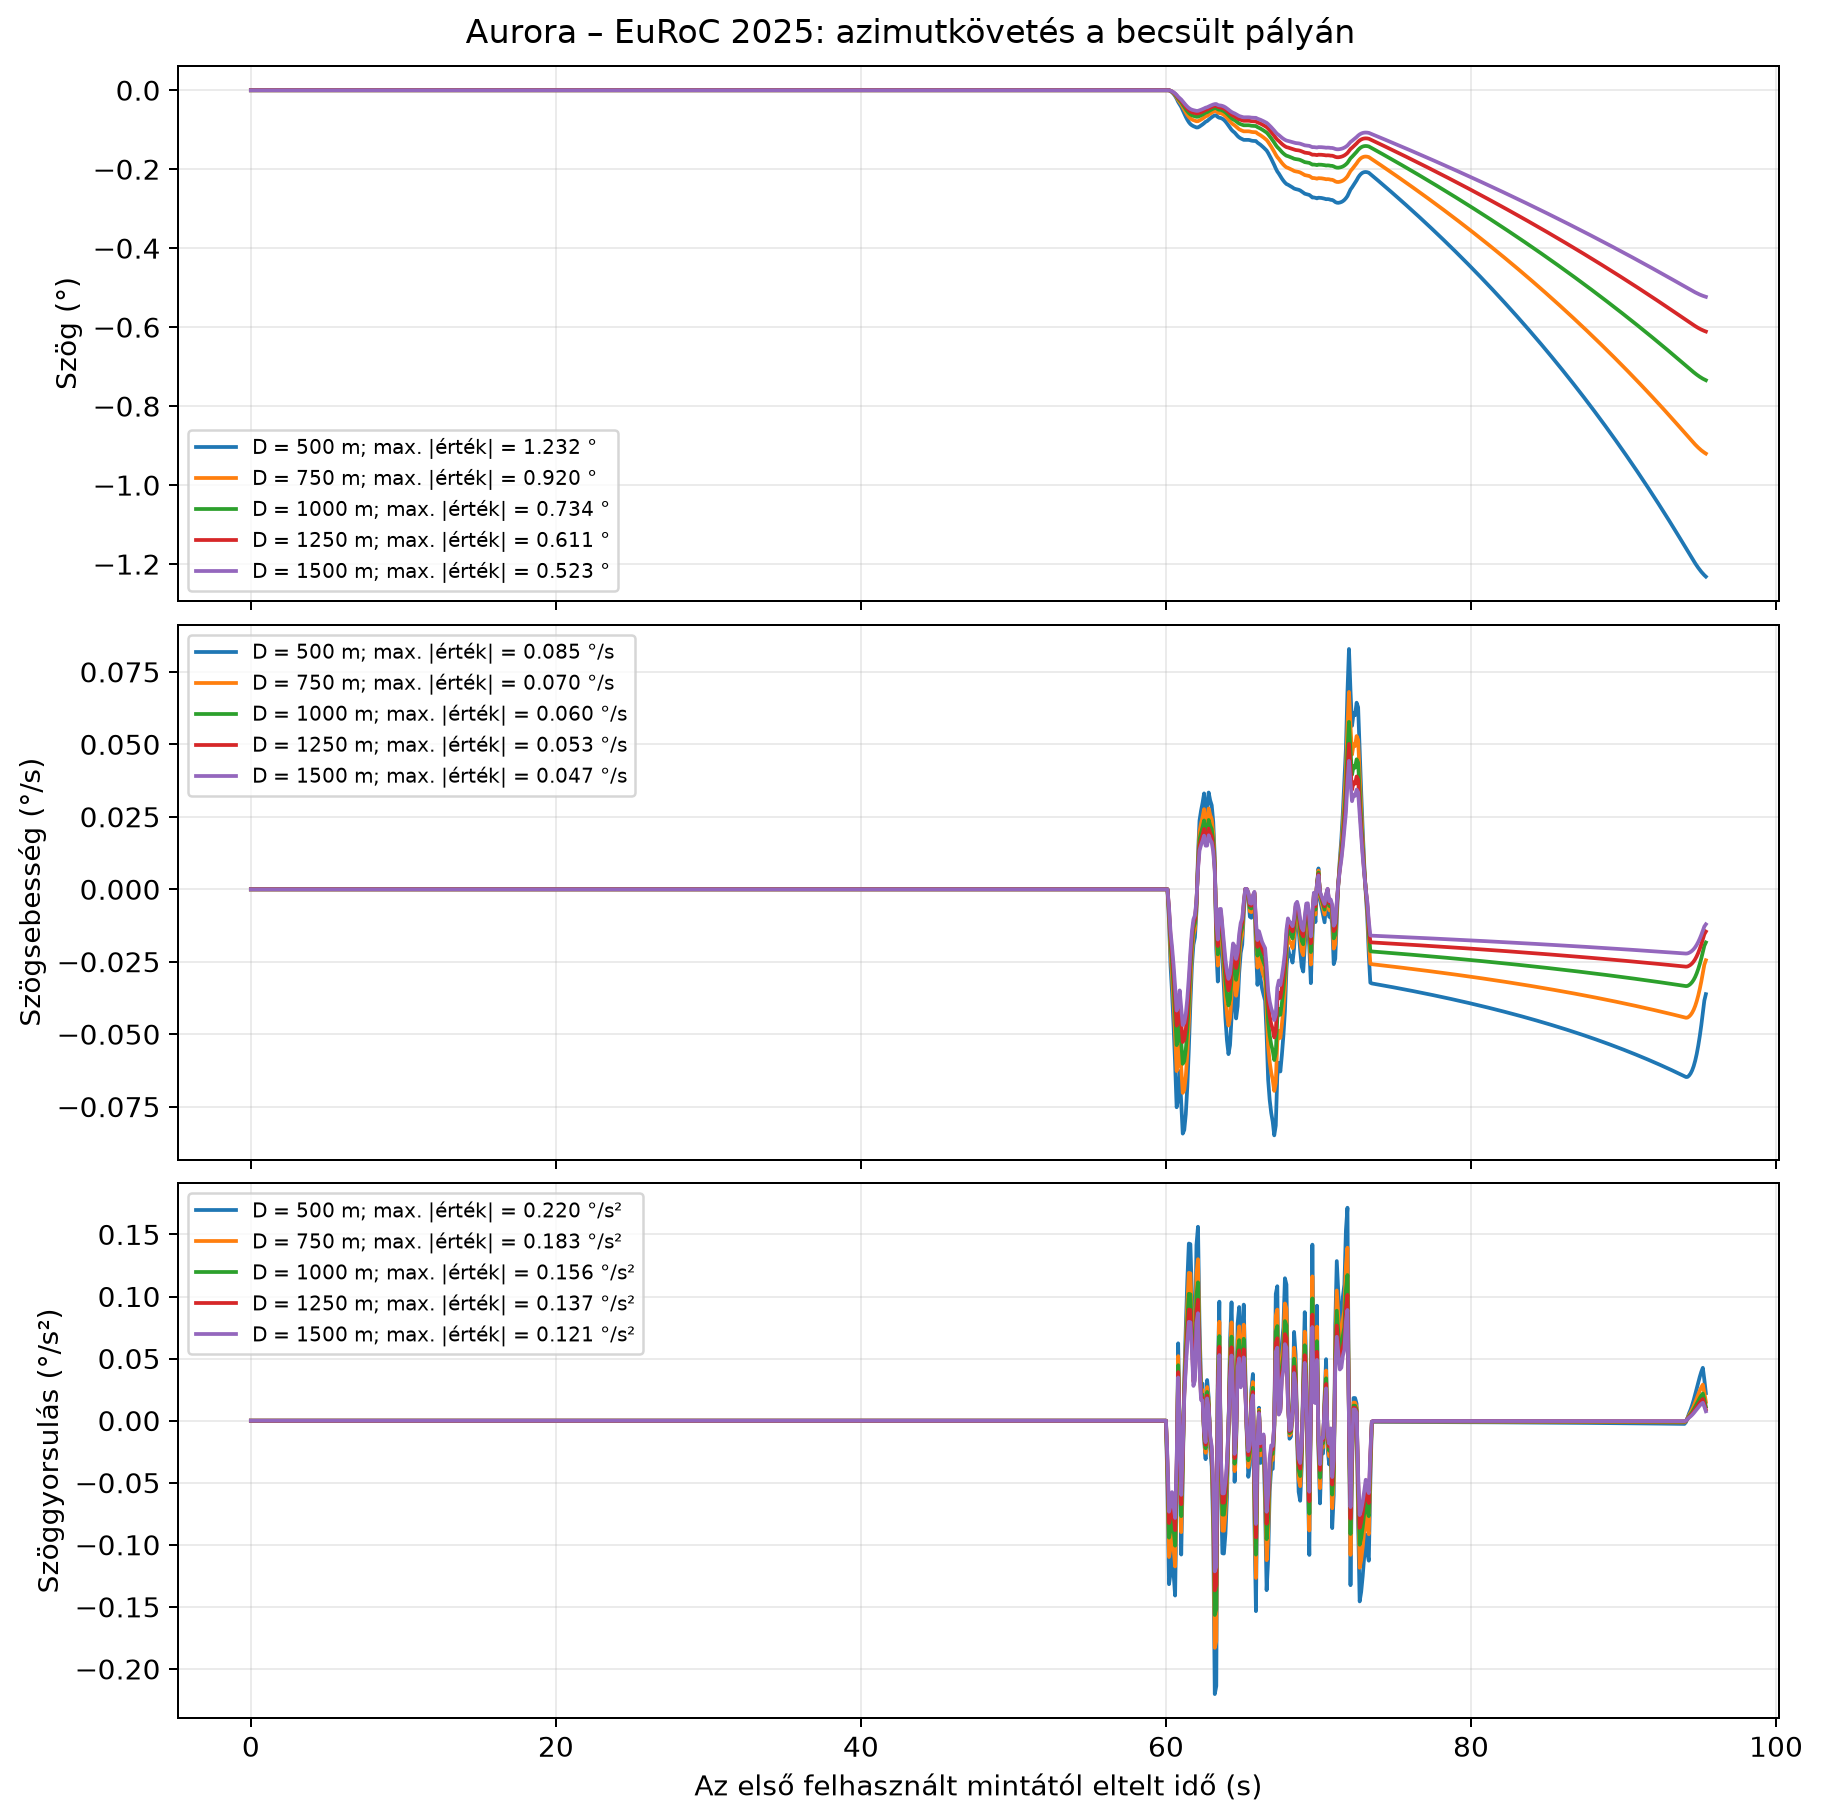
\includegraphics[width=\linewidth]{figures/Requirements/aurora_euroc_cats_azimuth_tracking.png}
        \captionsetup{width=\linewidth,format=plain,justification=centering}
        \caption{Az Aurora azimutkövetése a 2025-ös EuRoC során}
        \label{fig:aurora-euroc-cats-azim-tracking}
    \end{minipage}
\end{figure}



\subsubsection{Eredmények összefoglalása}
\ref{fig:eclipse-ift-elev-tracking} és \ref{fig:aurora-euroc-cats-elev-tracking}

A 2 repülési adat alapján a maximum elevációs szög, szögsebesség és szöggyorsulás az egyes
földi állomások esetén a következő táblázatban látható:
\begin{table}[H]
    \centering
    \caption{A két repülésből számított legnagyobb elevációs értékek a bázistávolság függvényében}
    \label{tab:kovetelmenyek-elevacio}
    \renewcommand{\arraystretch}{1.2}
    \begin{tabular}{|c|c|c|c|}
        \hline
        \rowcolor{blue!15}
        \textbf{$D$ (m)} & \textbf{Max. eleváció ($^\circ$)} & $\omega_{\max}$ ($^\circ$/s) & $\alpha_{\max}$ ($^\circ$/s$^2$) \\
        \hline
        500 & 72,52 & 12,59 & 6,69 \\
        \hline
        750 & 66,58 & 9,42 & 4,46 \\
        \hline
        1000 & 61,21 & 7,81 & 3,34 \\
        \hline
        1250 & 56,38 & 6,69 & 2,67 \\
        \hline
        1500 & 52,05 & 5,85 & 2,23 \\
        \hline
    \end{tabular}
\end{table}

\ref{fig:eclipse-ift-azim-tracking} és \ref{fig:aurora-euroc-cats-azim-tracking} grafikon alapján
A 2 repülési adat alapján a maximum azimut szög, szögsebesség és szöggyorsulás az egyes
földi állomások esetén a következő táblázatban látható:
\begin{table}[H]
    \centering
    \caption{A két repülésből számított legnagyobb azimutértékek a bázistávolság függvényében}
    \label{tab:kovetelmenyek-azimut}
    \renewcommand{\arraystretch}{1.2}
    \begin{tabular}{|c|c|c|c|}
        \hline
        \rowcolor{blue!15}
        \textbf{$D$ (m)} & \textbf{Max. azimutkitérés ($^\circ$)} & $\omega_{\max}$ ($^\circ$/s) & $\alpha_{\max}$ ($^\circ$/s$^2$) \\
        \hline
        500 & 25,07 & 2,57 & 3,03 \\
        \hline
        750 & 19,99 & 1,83 & 2,34 \\
        \hline
        1000 & 16,57 & 1,42 & 1,88 \\
        \hline
        1250 & 14,13 & 1,17 & 1,57 \\
        \hline
        1500 & 12,32 & 0,99 & 1,34 \\
        \hline
    \end{tabular}
\end{table}

A régebbi fellövések tapasztalatai alapján a földi állomás biztonsági távolsága
a rakétától minimum 1 km, így a továbbiakban a 750~m es távolsággal lesz számolva, hogy
azon belül biztosan meglegegyen. \\

Így a \ref{tab:kovetelmenyek-elevacio} és \ref{tab:kovetelmenyek-azimut} táblázatok alapján a
maximum értékek 750~m állomásgtávolság esetén a következőek 2-es biztonsági tényezővel számolva
a szögsebesség és szöggyorsulás követelményekre:

\begin{table}[H]
    \centering
    \caption{A követőmechanika tervezési követelményei tengelyenként ($D = 750$~m, $S = 2$)}
    \label{tab:tervezesi-kovetelmenyek-750m}
    \renewcommand{\arraystretch}{1.2}
    \begin{tabular}{|l|c|c|c|c|}
        \hline
        \rowcolor{blue!15}
        \textbf{Tengely} & $\omega_{\max}$ ($^\circ$/s) & $S\omega_{\max}$ ($^\circ$/s) & $\alpha_{\max}$ ($^\circ$/s$^2$) & $S\alpha_{\max}$ ($^\circ$/s$^2$) \\
        \hline
        Eleváció & 9,42 & \textbf{18,84} & 4,46 & \textbf{8,92} \\
        \hline
        Azimut & 1,83 & \textbf{3,66} & 2,34 & \textbf{4,68} \\
        \hline
    \end{tabular}
\end{table}

A tervezési szögsebesség az elevációs tengelyen
3,14~RPM, az azimuttengelyen pedig
0,61~RPM-nek felel meg.

Az antennák által lekövethtő maximális szögelfordulás, pedig tapasztalati úton lett meghatározva.
Az elavációs tengelyen pozitív tartományba képes legyen a követő antenna legalább 85 fokot pozitív irányba és -10 fokot
negatív irányba elfordulni, míg az azimut tengelyen mindkét irányba legalább 60 fokot elfordulni.
Ezek a követelmények a földi állomás esetleg magasabb elhelyezkedése és esetleges korai főernyőnyitás
és az ebből adódó nagyobb sodródási távolságok miatt lettek meghatározva. 

\subsection{Szükséges hajtónyomaték meghatározása}
A hajtónyomaték becslése egy 433~MHz-en használt Yagi
antennára és egy 2,4~GHz-es parabolikus antennára készült.
A vizsgált DIPOL ATK~10 a versenycsapat által eddig használt
legnagyobb antenna. Az ALFA AGA-2424T parabolikus antenna
egy későbbi bővítési lehetőség.

A parabolikus antennák általában nagyobb nyereséget
biztosítanak, azonban kisebb nyílásszögűek.
A vizsgált parabolikus antenna nyeresége 12~dB-lel
nagyobb a Yagi antennáénál. A parabolikus antenna
vízszintes és függőleges nyílásszöge rendre $14^\circ$
és $10^\circ$, a Yagi antennáé pedig $52^\circ$ és
$42^\circ$~\cite{parabolic-antenna,yagi-antenna}.
A keskenyebb nyaláb pontosabb irányzást igényel, ami
megnehezíti a kézi követést. A fejlesztett követőrendszer
egyik lehetséges alkalmazása ezért a parabolikus antenna
automatikus irányzása.


\subsubsection{Yagi antenna tehetetlenségi nyomatékának becslése}
A számítás alapjául szolgáló antennaadatok és
modellfeltevések:
\begin{itemize}
    \item Az antenna hossza 1,4~m, tömege 0,8~kg
          \cite{yagi-antenna}.
    \item Az antenna befoglaló méretei a hossztengelyre
          merőleges síkban: $290 \times 440$~mm
          \cite{yagi-antenna}.
    \item Az antenna egyenletes tömegeloszlású rúddal
          közelíthető.
    \item A rúd a végén van befogva.
\end{itemize}

Vízszintes antennahelyzetben mindkét forgástengely
merőleges a rúd hossztengelyére.
Az erre a helyzetre becsült tehetetlenségi nyomaték
mindkét tengelyre $J_{\mathrm{Yagi}}$
\cite{tehetetlensegi-nyom}:
\begin{equation}
    J_{\mathrm{Yagi}}=\frac{1}{3}ml^2=\frac{1}{3}\cdot0{,}8\cdot1{,}4^2\approx0{,}523~\mathrm{kg\cdot m^2}
\end{equation}

A gyorsítónyomaték számításához a
\ref{tab:tervezesi-kovetelmenyek-750m}.~táblázat tervezési
szöggyorsulásait radián per másodpercnégyzetre átváltva:
\begin{align}
    M_{\mathrm{gyors,El}} &= J_{\mathrm{Yagi}}\alpha_{\mathrm{El}} \approx 0{,}523\cdot 8{,}92\cdot\frac{\pi}{180}\approx 0{,}081~\mathrm{Nm} \\
    M_{\mathrm{gyors,Az}} &= J_{\mathrm{Yagi}}\alpha_{\mathrm{Az}} \approx 0{,}523\cdot 4{,}68\cdot\frac{\pi}{180}\approx 0{,}043~\mathrm{Nm}
\end{align}

A szél hatásának becslésekor, 6~m/s-os szélsebesség van alapul véve,
mivel erős szélben a fellövést elhalasztják. 
A vizsgált esetben a szél az antenna oldalfelületére merőlegesen hat,
mert így adódik a legnagyobb azimutirányú szélnyomaték.
A számítás az antenna vetületi felületét tömör síklapként
veszi figyelembe, $C_d=1{,}28$ légellenállási tényezővel.
A vetületi felület az 1,4~m-es rúdhossz és a 0,29~m-es
befoglaló magasság szorzata.
A szélerő így a következőképpen számítható:
\begin{equation}
    F_{\mathrm{szél}}
    = \frac{1}{2}\rho v^2C_d A_{\mathrm{vet}}
    = \frac{1}{2}\cdot1{,}225\cdot6^2\cdot1{,}28
      \cdot(1{,}4\cdot0{,}29)
    \approx 11{,}46~\mathrm{N}
\end{equation}
Egyenletes terhelés esetén az eredő szélerő a rúd
közepén, a forgástengelytől 0,7~m-re hat:
\begin{equation}
    M_{\mathrm{szél,Az}}
    = F_{\mathrm{szél}}\cdot0{,}7
    \approx 8{,}02~\mathrm{Nm}
\end{equation}
Az elevációs szélnyomatékra ez a terhelési eset nem terjed ki. \\

A gravitáció a függőleges azimuttengely körül nem fejt
ki forgatónyomatékot. Az elevációs tengely körül a
gravitációs nyomaték vízszintes antennahelyzetben a
legnagyobb. Ekkor a rúdmodellben a súlyerő erőkarja
a rúd hosszának fele, $d=0{,}7~\mathrm{m}$:
\begin{equation}
    M_{\mathrm{grav,El}}=mgd=0{,}8\cdot9{,}81\cdot0{,}7\approx5{,}494~\mathrm{Nm}
\end{equation}

A Yagi antenna becsült hajtónyomatéka a figyelembe vett
terhelések összege:
\begin{align}
    M_{\mathrm{hajt,El}} &= M_{\mathrm{gyors,El}}+M_{\mathrm{grav,El}}
    \approx 5{,}575~\mathrm{Nm} \\
    M_{\mathrm{hajt,Az}} &= M_{\mathrm{gyors,Az}}+M_{\mathrm{szél,Az}}
    \approx 8{,}06~\mathrm{Nm}
\end{align}



\subsubsection{Parabolikus antenna tehetetlenségi nyomatékának becslése}
A számítás alapjául szolgáló antennaadatok és modellfeltevések:
\begin{itemize}
    \item Az ALFA AGA-2424T antenna tömege 2,8~kg,
          befoglaló mérete $600 \times 900$~mm
          \cite{parabolic-antenna}.
    \item Az antenna egyenletes tömegeloszlású,
          $a=0{,}6~\mathrm{m}$ széles és
          $b=0{,}9~\mathrm{m}$ magas téglalapként közelíthető.
    \item Az azimuttengely a tömegközépponton halad át.
          Az elevációs tengely távolsága a tömegközépponttól
          a becslésben $l=0{,}2~\mathrm{m}$.
\end{itemize}

Az elevációs tengelyre a Steiner-tétellel, az
azimuttengelyre a tömegközépponton átmenő tengelyre
vonatkozó összefüggéssel adódik a tehetetlenségi nyomaték:
\begin{align}
    J_{\mathrm{El}} &= \frac{1}{12}mb^2 + ml^2
                    = 0{,}301~\mathrm{kg\cdot m^2} \\
    J_{\mathrm{Az}} &= \frac{1}{12}ma^2
                    = 0{,}084~\mathrm{kg\cdot m^2}
\end{align}

A Yagi antennához hasonlóan a gyorsítónyomaték
a tehetetlenségi nyomaték és a tervezési szöggyorsulás
szorzata:
\begin{align}
    M_{\mathrm{gyors,El}} &= J_{\mathrm{El}}\alpha_{\mathrm{El}}
    = 0{,}301\cdot 8{,}92\cdot\frac{\pi}{180}
    \approx 0{,}047~\mathrm{Nm} \\
    M_{\mathrm{gyors,Az}} &= J_{\mathrm{Az}}\alpha_{\mathrm{Az}}
    = 0{,}084\cdot 4{,}68\cdot\frac{\pi}{180}
    \approx 0{,}007~\mathrm{Nm}
\end{align}


A szélterhelés nagysága az elöző fejezethez hasonlóan,
6~m/s szélsebesség esetén lett becsülve, amely
a parabolikus antenna vetületi felületére merőlegesen hat
és $C_d=1{,}28$ légellenállási tényezővel véve.

A rácsos antenna effektív felületének becsléséhez a
befoglaló felület 65\%-a szolgált alapul:
\begin{equation}
    A_{\mathrm{eff}} = 0{,}65\,ab = 0{,}351~\mathrm{m^2}
\end{equation}

Az azimutirányú szélnyomaték becslése egyoldali terheléssel
készült. A szél az antennafelületnek csak az azimuttengely
egyik oldalán lévő felére hat.
Az erre a fél felületre jutó eredő szélerő nagysága:
\begin{equation}
    F_{\mathrm{egyen,szél}}
    = \frac{1}{2}\rho v^2 C_d\frac{A_{\mathrm{eff}}}{2}
    \approx 4{,}953~\mathrm{N}
    \label{eq:szel-egyenerteku}
\end{equation}

Az eredő szélerő a terhelt fél felület középpontjában hat,
az azimut tengelytől $a/4$ távolságra, így az azimutirányú szélnyomaték:
\begin{equation}
    M_{\mathrm{szél,Az}}
    = F_{\mathrm{egyen,szél}}\frac{a}{4}
    \approx 0{,}743~\mathrm{Nm}
\end{equation}
Az elevációs szélnyomaték a parabolikus antenna becslésében
sem szerepel.

A gravitációs nyomaték a függőleges azimuttengely körül nulla.
Az elevációs tengely körül akkor adódik a legnagyobb
gravitációs nyomaték, amikor a súlyerő erőkarja eléri
a korábban megadott $l=0{,}2~\mathrm{m}$ értéket:
\begin{equation}
    M_{\mathrm{grav,El}}=mgl=2{,}8\cdot9{,}81\cdot0{,}2\approx5{,}494~\mathrm{Nm}
\end{equation}

A hajtónyomaték becslése az elevációs tengelyen a gyorsítás
és a gravitáció, az azimuttengelyen pedig a gyorsítás és a
szélterhelés hatásá mellett:
\begin{align}
    M_{\mathrm{hajt,El}} &= M_{\mathrm{grav,El}}+M_{\mathrm{gyors,El}}
    \approx5{,}54~\mathrm{Nm} \\
    M_{\mathrm{hajt,Az}} &= M_{\mathrm{szél,Az}}+M_{\mathrm{gyors,Az}}\approx0{,}743+0{,}007=0{,}750~\mathrm{Nm}
\end{align}



\subsubsection{Összesítés}
A két antenna tengelyenként becsült hajtónyomatékát
a \ref{tab:hajtonyomatek-osszesites}.~táblázat foglalja össze.

\begin{table}[H]
    \centering
    \caption{A becsült hajtónyomaték az antenna forgástengelyein}
    \label{tab:hajtonyomatek-osszesites}
    \renewcommand{\arraystretch}{1.2}
    \begin{tabular}{|l|c|c|}
        \hline
        \rowcolor{blue!15}
        \textbf{Antenna} & \textbf{Eleváció} (N\,m)
                         & \textbf{Azimut} (N\,m) \\
        \hline
        DIPOL ATK~10 & 5,575 & 8,06 \\
        \hline
        ALFA AGA-2424T & 5,54 & 0,750 \\
        \hline
    \end{tabular}
\end{table}

A hajtás kiválasztásához tengelyenként a két antennára
becsült nyomatékigény közül a nagyobb érték szolgált
alapul. Ez az elevációs tengelyen $5{,}575~\mathrm{Nm}$,
az azimuttengelyen pedig $8{,}06~\mathrm{Nm}$.

A szükséges tengelynyomaték megfelelő áttétellel is
elérhető. A lassító áttétel növeli a kimeneti nyomatékot,
miközben csökkenti a kimeneti fordulatszámot. Ezért
olyan motor és áttétel szükséges, amellyel az antenna
tengelyén a szükséges nyomaték és a tervezési
szögsebesség egyszerre biztosítható.

\subsection{Érzékelési és visszacsatolási követelmények}

A fejlesztés célja olyan vezérlőelektronika kialakítása, amely lehetővé teszi
a az antennakövető algoritmusok késöbbi fejlesztését és tesztelését.
Ehhez biztonosítani kell a vezérlő elektronika számára a motorok
vezérlését, az antenna szöghelyzetének és szögsebességének visszacsatolását 
és a követőállomás saját helyzetének meghatározását.
A visszacsatolás mellett fogadnia kell a rakétáról érkező helyzet, sebesség
és gyorsulás adatokat.

A követési pontosság meghatározásánál, a mérvadó a vizsgált antennák nyílásszöge,
amelyek közül a kisebb a parabolikus antenna.
A parabolaantenna nyílásszöge vízszintesen $14^\circ$, 
függőlegesen $10^\circ$ \cite{parabolic-antenna}. 
Így a félnyílásszögeket figyelembe véve az antenna tényleges irányának
maximális megengedett követési hiba az azimut tengelyen $7^\circ$ fok, míg
az elevációs tengelyen $5^\circ$ fok. 

A követési hibához a kezdeti helymeghatározás és szögérzékelés hibája, mechanikai
pontatlanságok valamint a szabályzából adódó hibák is hozzájárulnak. Emiatt az érzékelők
pontossági követelményeit úgy kell meghatározni, hogy a megengedett eltérés 
kis része származzon a mérési hibákból. Így nagyobb tartalék marad a mechanikai és
szabályozási pontatlanságokból adódó hibákra.


\subsubsection{Antenna orientációjának érzékelése}
\label{Req-Antenna-Orientacio}
\textcolor{red}{https://www.rfhamdesign.com/downloads/spx-06-azel-specifications-sheet.pdf}
\textcolor{red}{https://repositum.tuwien.at/handle/20.500.12708/13686}
\textcolor{red}{\url{https://www.safran-group.com/sites/default/files/2023-10/Safran_Data_Systems-Sparte_300_Antenna-Product_Summary.pdf}}
\textcolor{red}{https://www.nasa.gov/wp-content/uploads/2015/03/sounding-rocket-user-handbook.pdf}

Bekapcsoláskor a rendszernek meg kell határozni a kezdeti azimut és elevációs szöget,
legfeljebb $1~^\circ$ pontossággal.
Ezek a szögek adják a referenciát az antenna késöbbi szöghelyzetének meghatározásához.

A működés közbeni visszacsatolsához mindkét tengelyen érzékelni kell az antenna 
szögelfordulását. Hasonló antennakövető rendszereknél ez a felbontás
$0,1~^\circ$ és $0,01~^\circ$ felbontás között változik \textcolor{red}{LINK}. 
Ezek alapján a tervezett rendszerben már a $0,1~^\circ$ antennaelfordulás
érzékelése is szükséges. A mért szöghelyzet időbeli változásából
a szögsebesség és a szöggyorsulás is meghatrozható.

\subsubsection{Földi követőállomás helyének meghatározása}
Az antenna célirányát a követőállomástól a rakéta felé mutató,
\eqref{eq:kovetes-relativ-pozicio} szerinti relatív helyvektor
határozza meg. Ennek kiszámításához a rakéta telemetrián érkező
helyzetadatai mellett a követőállomás földrajzi koordinátái és
magassága is szükséges. A követőállomás ezért szükséges egy 
saját helymeghatározó rendszerrel rendelkezzen. Ebből
elketerülhetőek a bevitelből adódó hibák, valamint automatizálja
a rendszer működését.

A repülés során a földi állomás helyzete konstans, így a helymeghatározó eszköz
vevési ideje nem egy kritikus paraméter. Azonban mind az azimuth
tengely és az elevációs tengely szögének pontosságát befolyásolja a vevő pontossága. 
Egy 5~m magassági és vízszintes pontosságú  vevő esetén a 750~m távolságra lévő rakéta
a fellépő elevációs és azimuth szöghiba a két tengelyen azonos, amely 
a következőképpen számítható: 
\begin{equation}
    |\Delta\psi| = |\Delta\theta|
    = \arctan\!\left(\frac{5}{750}\right)
    \approx 0{,}38^\circ
\end{equation}

\subsection{Összesítés}
A vizsgált kezdeti helyzetben a kezdőirány és a helymeghatározás
hibája azonos irányú eltérés esetén tengelyenként összesen
$1^\circ + 0{,}38^\circ = 1{,}38^\circ$. Így azimutban
$5{,}62^\circ$, elevációban pedig $3{,}62^\circ$ marad a követés
során fellépő további hibákra.

Emellett a szöghelyzet visszacsatolásának felbontása legalább $0{,}1^\circ$ 
felbontású kell hogy legyen, hogy a szabályozó már ekkora
elfordulást is érzékelhessen.

\subsection{Interfész követelmények}
A vezérlőelektronikának biztosítani kell a kétirányú adatátvitel
a földi állomás számotógép és az irányító elektronika között,
valamint a rakéta telemetriai adatainak fogadását és feldolgozását a 
csatlakoztaott rádiómodulokon keresztül. 
Késöbbi bővítésekhez külső érzékelőmodulok csatlakoztatására és
tápellátására is lehetőséget kell biztosítani.

\subsubsection{Kommunikáció a földi állomással}
A vezérlőelektronika és a földi állomás számítógépe között
USB~2.0 interfészen kell biztosítani a kétirányú adatátvitelt.
Ezen a kapcsolaton keresztül a vezérlőparancsokat 
küldhet a követőállomásnak, valamint kiolvasja a 
a követés alatt mért adatokat valamint a rakétáról fogadott telemetriai adatokat.

\subsubsection{Kapcsolat a telemetria feldolgozó egységgel}
\label{subsubsec:req-kapcsolat-telem}
A rádiómodulok típustól függően áltálában SPI vagy UART kommunikációs protokolt használnak
a mikrovezérlővel való kommunikációhoz. 
A versenycsapat által néhány már használt modulok közül
LoRa128xf27 SPI interfészen, míg a E32-433T30D pedig UART interfészen keresztül
kommunikál\cite{lora128xf27} \cite{e32-433t30d}. A vezérlőelektronikán ezért 
külön SPI és UART-csatlakozót kell biztosítani, hogy mindkét típus csatlakoztatható legyen. 
\textcolor{red}{elbasztam a huzalozást 4 adatjelnek kéne lennie; de én csak DIO1-ig vittem ki vmiért}

A modulok 5~V-os tápellátást igényelnek, amelyet a vezérlőelektronika biztosít.
Ezeknek a telemetria moduloknak az áramfelvétele működéstől függen változhat,
azonban a maximális áramfelvételük az E32-433T30D esetén 610~mA, a LoRa128xf27 
esetén pedig 600~mA. 
Emiatt a vezérlőelektronikának biztosítani kell egy legalább tartalékkal együtt
1~A terheltőségű 5~V-os tápellátást csak telemetria modulok számára.

\subsubsection{Bővítési lehetőségek}
\label{subsubsec:req-bovitesi-lehetosegek}
A vezérlőelektronikának lehetőséget kell biztosítani jövőbeli bővítésekhez,
például egy külső időjárás állomás panel csatlakozásához, amely a környezeti hőmérsékletet,
páratartalmat, szélsebességet és szélirányt mérve biztosítja a földi állomás számára a
rakéta követéshez szükséges környezeti adatokat. 

A bővítéshez általáns célú duplex adatátvitelre képes kommunikációs protokollt kell biztosítani.
Ehhez jelenleg a hardveres egyszerűsége miatt az I2C protokoll lett kiválasztva,
amely lehetőséget biztosít több eszköz csatlakozására és kezelésére is. \textcolor{red}{ezt nem 
ide hanem a hardveres reszbe?} \\

A kommunikációs kimenetek mellett szükséges a megfelelő tápellátás biztosítása is,
amelyre egy maximális 1~A áramfelvételű 5~V-os tápellátást biztosító kimenet lett meghatározva.
Ez szinte minden szenzor bővítéshez elegendő, illetve kis alapvető aktuátorok meghajtásához
is elegendő. 

\subsection{Adattárolási követelmények}
\label{subsec:req-adattarolas}
A követőállomás működésének utólagos kiértékeléshez és 
redundancia biztosításához nagy kapacitású, kivehető adattárolóra
van szüksége. A rakáta telemetriai adatainak, a követőállomásnak
küldött parancsok valamint a követés során mért adatok, állapotok és
számított irány mentése is szükséges. A különböző mentett adatokhoz
időbélyegek is szükségesek hogy összevethetőek legyenek.
A kivehető adattároló lehetővé teszi a mentett adatok egyszerűvé
teszik a mentett adatok utólagos feldolgozását.

Az adott antennához tartozó kalibrációs értékeket a panelre elhelyezett,
nem kivehető és nem felejtő memóriába kell tárolni, hogy 
függetlenül a kivehető adattárolótol a rendszer működésre álljanak.
Ha a kivehető tároló nincsen benne a rendszerbe mint korlátozott
mennyiségű adattárolására is alkalmasnak kell lennie.
\textcolor{red}{konkrét mennyiséget meghatározni?}

\subsection{Tápellátási követelmények}
\label{subsec:req-aramfelvetel}
A tápellátás méretezésének alapját a korábban meghatározott
interfészkövetelmények és a \ref{chap:elektronikai-hardver}.~fejezetben
bemutatott hardverfelépítés adja. A rádiómodulok és a bővítőcsatlakozó
áramigényét az előírt terhelhetőség, a hajtásokét a kiválasztott
motorok adatai, a vezérlőelektronikáét pedig a tervezett kapcsolás
alapján lehet megbecsülni.

A kiválasztott motorok 12~V-os tápfeszültséggel működnek \ref{subsec:motorok-kiválasztása}.
Így a vezérlőelektronika 12~V-os tápellátást igényel bemeneti feszültségként, 
és ebből állítja elő az elektronika ellátásához szükséges 5~V-ot.
A hajtások maximális áramigényét a \ref{tab:motor-parameterek}.~táblázatban
megadott motoradatok alapján lehet meghatározni. Egy motor
blokkolási árama legfeljebb 10~A, így a két motor
egyidejű blokkolását feltételezve a hajtások méretezési árama
20~A.

Az 5~V-os ágon a rádiómodulok közös tápellátására 1~A, a
bővítőcsatlakozóra további 1~A jut a
\ref{subsubsec:req-kapcsolat-telem}. és a
\ref{subsubsec:req-bovitesi-lehetosegek}.~alfejezetben meghatározott
követelmények alapján. A vezérlőelektronika és az érzékelők
ellátására együttesen további 1~A-rel számolva a három áramkeret
összege 3~A. Az 5~V-os tápág választott terhelhetősége 5~A,
ami ehhez képest 2~A tervezési tartalékot biztosít.

Az 5~V-os tápág teljes terhelése 25~W kimeneti teljesítménynek
felel meg. A feszültségátalakítóra 90\%-os hatásfokot
feltételezve a teljes rendszer 12~V-os bemenetére adódó
méretezési áram
\begin{equation}
    I_{\mathrm{be}}
    = 2 \cdot 10~\mathrm{A}
    + \frac{5~\mathrm{V} \cdot 5~\mathrm{A}}
           {12~\mathrm{V} \cdot 0{,}9}
    \approx 22{,}31~\mathrm{A}
\end{equation}

Ennek alapján a 12~V-os bemeneti tápút rövid idejű
méretezési árama felfelé kerekítve 23~A.
\textcolor{red}{Ez mennyire eroltetet, ez is meg lett mar hatarozva elobb...}

% ------------------------------------------------------------------
\section{Rendszerarchitektúra}
% ------------------------------------------------------------------

A követőállomás vezérlőelektronikája 
felépítse két panelre tagoldóik. A központi vezérlőpanel az 
adatfeldolgozásért, szenzorok kezeléséért, a kommunikációt, valamint a vezérlő algoritmusok
futtatásáért és hajtások vezérléséért felelős.
A teljesítményelektronikai panel a két tengely 
motorjainak meghajtásáért és az elektronikai tápellátásáért felelős.

A kétpaneles kialakítás lehetővé teszi hogy a motorok
tápútjai és  meghajtóáramkörei a külön panelre kerüljenek,
ezzel csökkentve a vezérlőpanelre jutó zavarokat.
A két panel közötti kapcslatot táővezetékek, 
motorvezérlő jelek valamint a hajtás felöl jövő visszacsatoló jelek biztosítják.

\subsection{Rendszer áttekintése}

% Blokkvázlat 

\subsubsection{Központi vezérlőpanelek felépítése}
%vmi olyasmi h a kifejtese es az alkatreszvalasztsok majd abban az alfejezetben lesznek
% Blokkvázlat 


\subsubsection{Teljesítményelektronikai panel felépítése}

%Blokkvázlat

